\chapter{Prototype Systems}
\label{prototypes}

Over the past several years we have been working on the creation of a family of
child-friendly tangible user interfaces that would serve as input devices for
exploring 3D modeling and digital fabrication in an ``embodied'' fashion. As
discussed in the first chapter, the motivations behind this work are
thematically diverse, but can be distilled into an attempt to create a more
intuitive, body-centric way for novices to design for 3D printing while also
strengthening the user's sense of spatial translation from 3D to 2D (screen
based) representations. To this end, we have created three prototypes:
the UCube, an initial proof-of-concept device, SnapCAD, a more expressive and
capable iteration of the UCube, and PopCAD - a paper-based interface addressing
several of the cost and portability concerns raised by SnapCAD. These systems
all communicate with versions of a companion software program running on desktop
computer. This chapter describes (in chronological order) the development of
these three systems, the software that interfaces with them, the motivations
behind their design, and the technical work involved in their creation.

\section{UCube}

The UCube represents our first attempt to create a cooperative system of
hardware and software that encapsulated and combined our beliefs about embodied
cognition and the importance of accessible digital fabrication. The idea for the
UCube originally came from the attempt to create a ``3D Geoboard''.
\ref{fig:geoboard} shows a rudimentary 2D geoboard consisting of a 3x3 grid
of nails stuck into a wooden block. Simple geometries, such as the triangle shown
in the referenced image, can be made by stretching rubber bands around some
number of ``pegs''. The geoboard invites a kind of tangible, exploratory, and
embodied play that (as we discuss in Chapter 3) promotes children's learning in
powerful ways. The initial design goal was to capture the ``gestalt'' of
the traditional 2-dimensional geoboard and extend it - into 3-dimensions, and with a
computationally-enhanced interface that could translate physical manipulations
on a device into a software program that could display the actions performed on
the geoboard in a ``meaningful'' way - that is, in a way that could potentially
extend spatial reasoning abilities between the 3D representations created on
the device and the 2D, screen-based images displayed on the computer screen.

\begin{figure}[ht]
\begin{center}$
\begin{array}{cc}
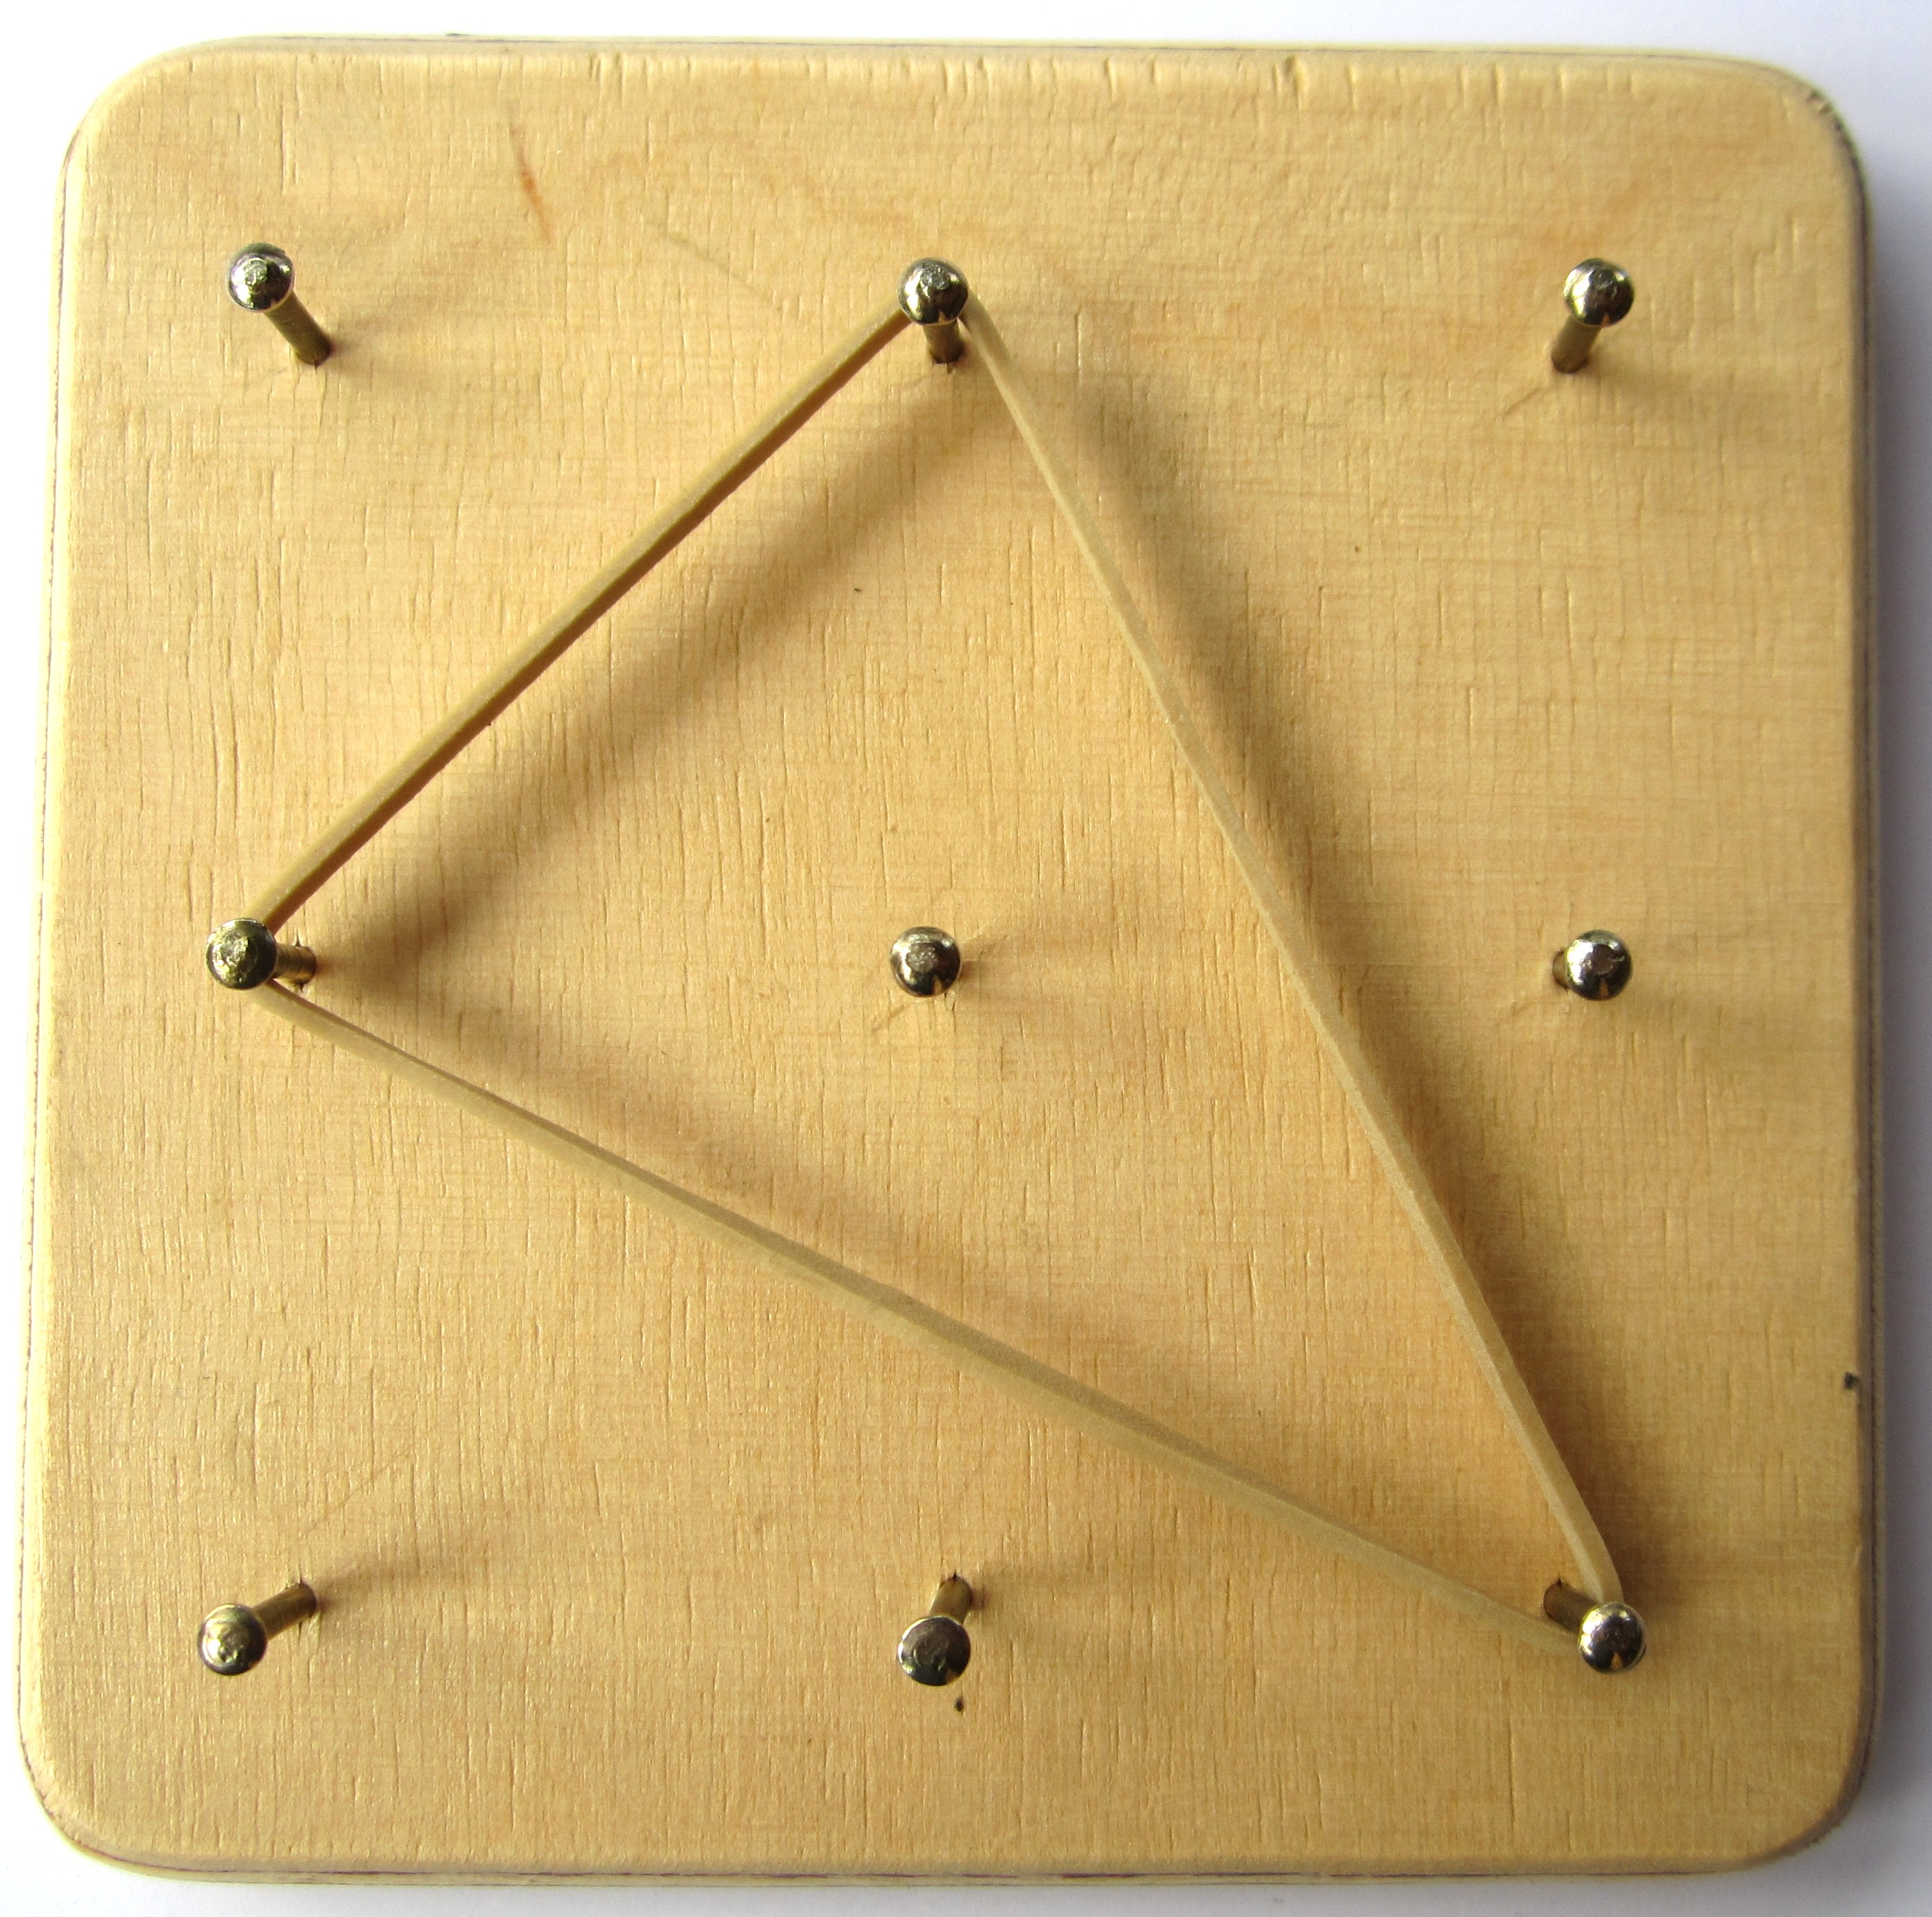
\includegraphics[width=.5\linewidth]{images/Geoboard}
\end{array}$
\end{center}
\caption{A simple 3x3 geoboard, with a rubber band stretched around several
pegs, forming a triangle.}
\label{fig:geoboard}
\end{figure}

The UCube (as seen on the left in \ref{fig:cubev1}) is the initial result of
this goal. The physical interface consists of a set of vertical ``towers'' that
are placed (and optionally re-placed) onto a grid of 4x4 evenly spaced nodes or
sockets into which the towers are placed, acting somewhat like the nails in the
2D geoboard. The towers themselves contain four switches placed vertically along
the tower, creating a potential for 64 (4x4x4) distinct points to be activated.
The towers are ``plugged in'' when placed into one of the 16 socket nodes,
connecting them to the underlying circuitry responsible for providing power to
the towers and relaying the state of each of the switches to the computer, via
an Arduino Mega\cite{ArduinoMega} microcontroller. Thus, when a tower is placed
in a specific node on the board and a switch is flipped on, a particular (x,y,z)
coordinate in three-dimensional space is activated and sent to a piece of
software on the computer. An abstracted illustration of the hardware system is
seen on the right in \ref{fig:ucube1_schematic}.

In turn, the UCube software (discussed more thoroughly later in the chapter)
takes the incoming coordinate data from the microcontroller and translates it
into a real-time visualization on screen. The graphical user interface centers
around a ``ghosted'' grid of all the potential points, with the active points
being highlighted. In the first version of the software, the interface also
provides a set of operations that can be performed on the set of active points
in addition to normal scene manipulations like zoom and rotate. These functions
include: taking the convex hull of the point set (as imagined in
\ref{fig:cubev1}), creating a sequential path or knot through the active points,
exporting the convex hull or knot to .STL format for 3D printing, drawing a
(non-printable) spline through the active points, saving and loading a shape,
and editing the vertices of a convex hull via a click-and-drag interface.


\begin{figure}[!ht]
\begin{center}$
\begin{array}{cc}
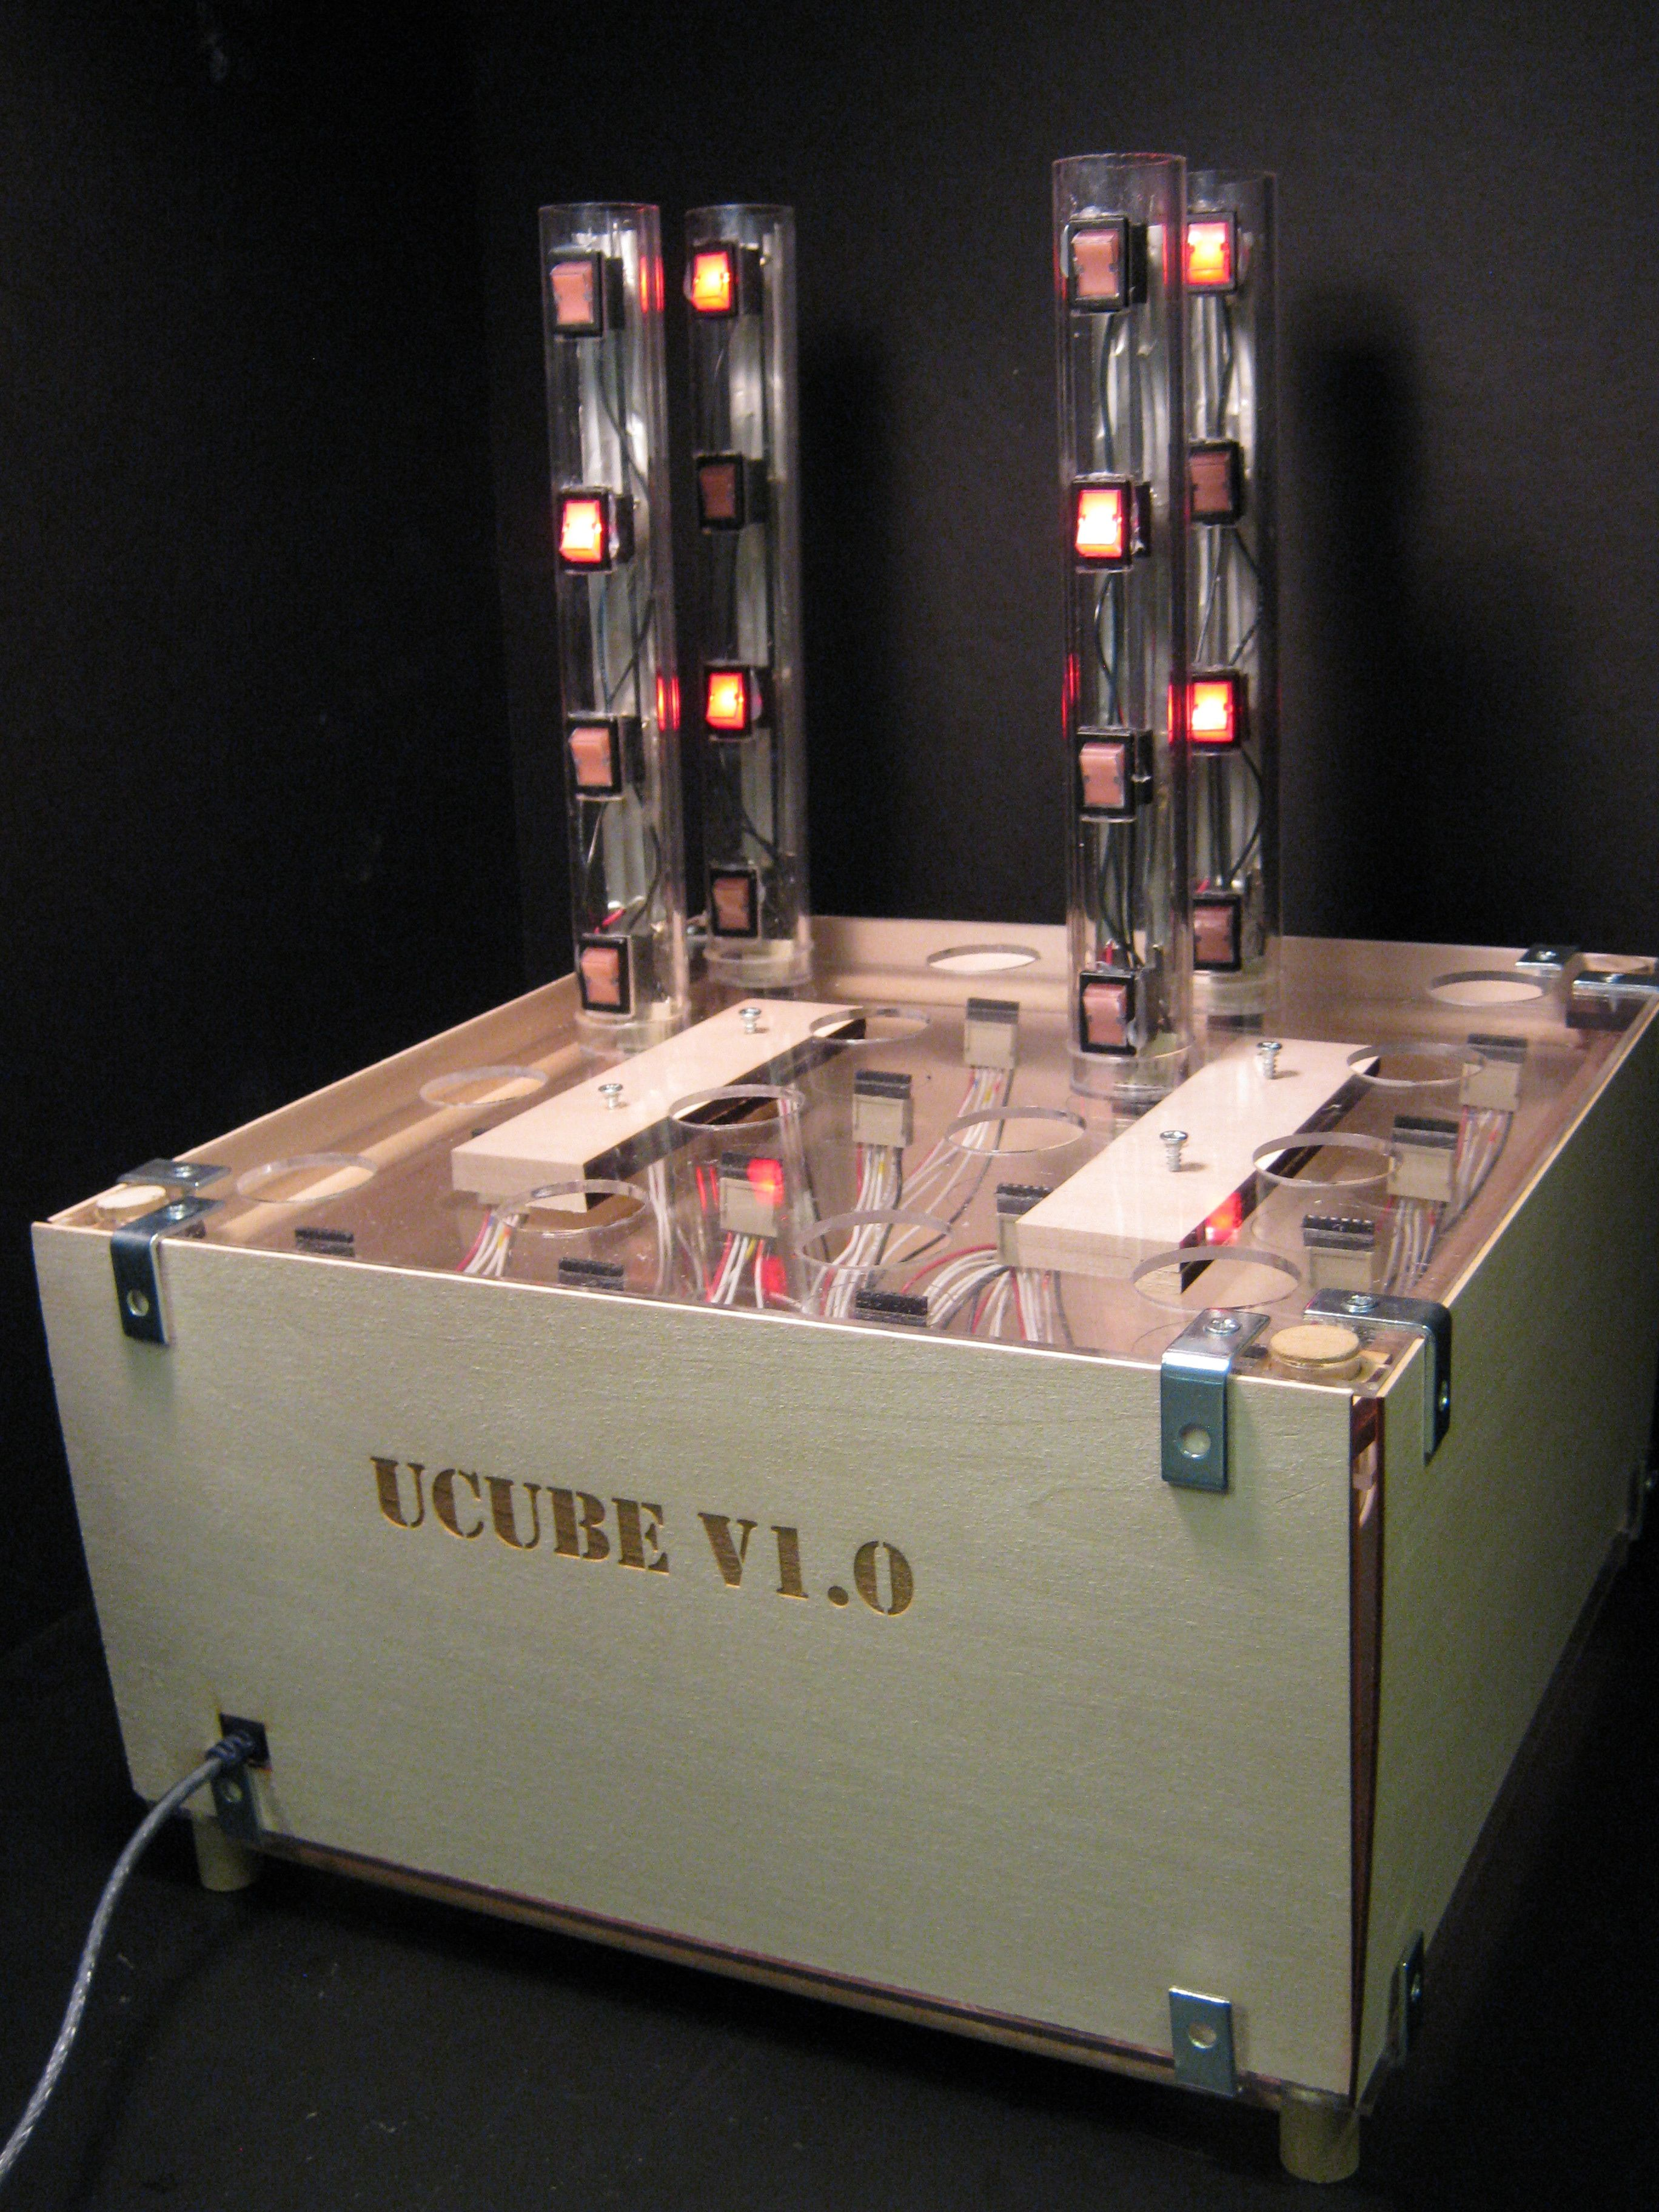
\includegraphics[width=.35\linewidth]{images/ucube1_triPrism}&
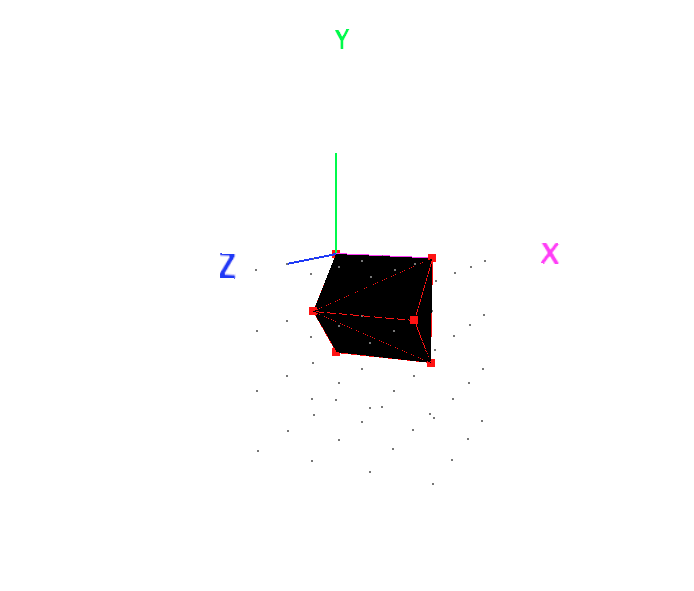
\includegraphics[width=.5\linewidth]{images/ucube1_software}
\end{array}$
\end{center}
\caption{Left: The UCube device, with four towers and six lit switches,
representing the six vertices of a triangular prism. Right: An early version of
the UCube software, representing the convex hull formed with the six active
points from the picture to the left.}
\label{fig:cubev1}
\end{figure}


\begin{figure}[!ht]
\begin{center}$
\begin{array}{cc}
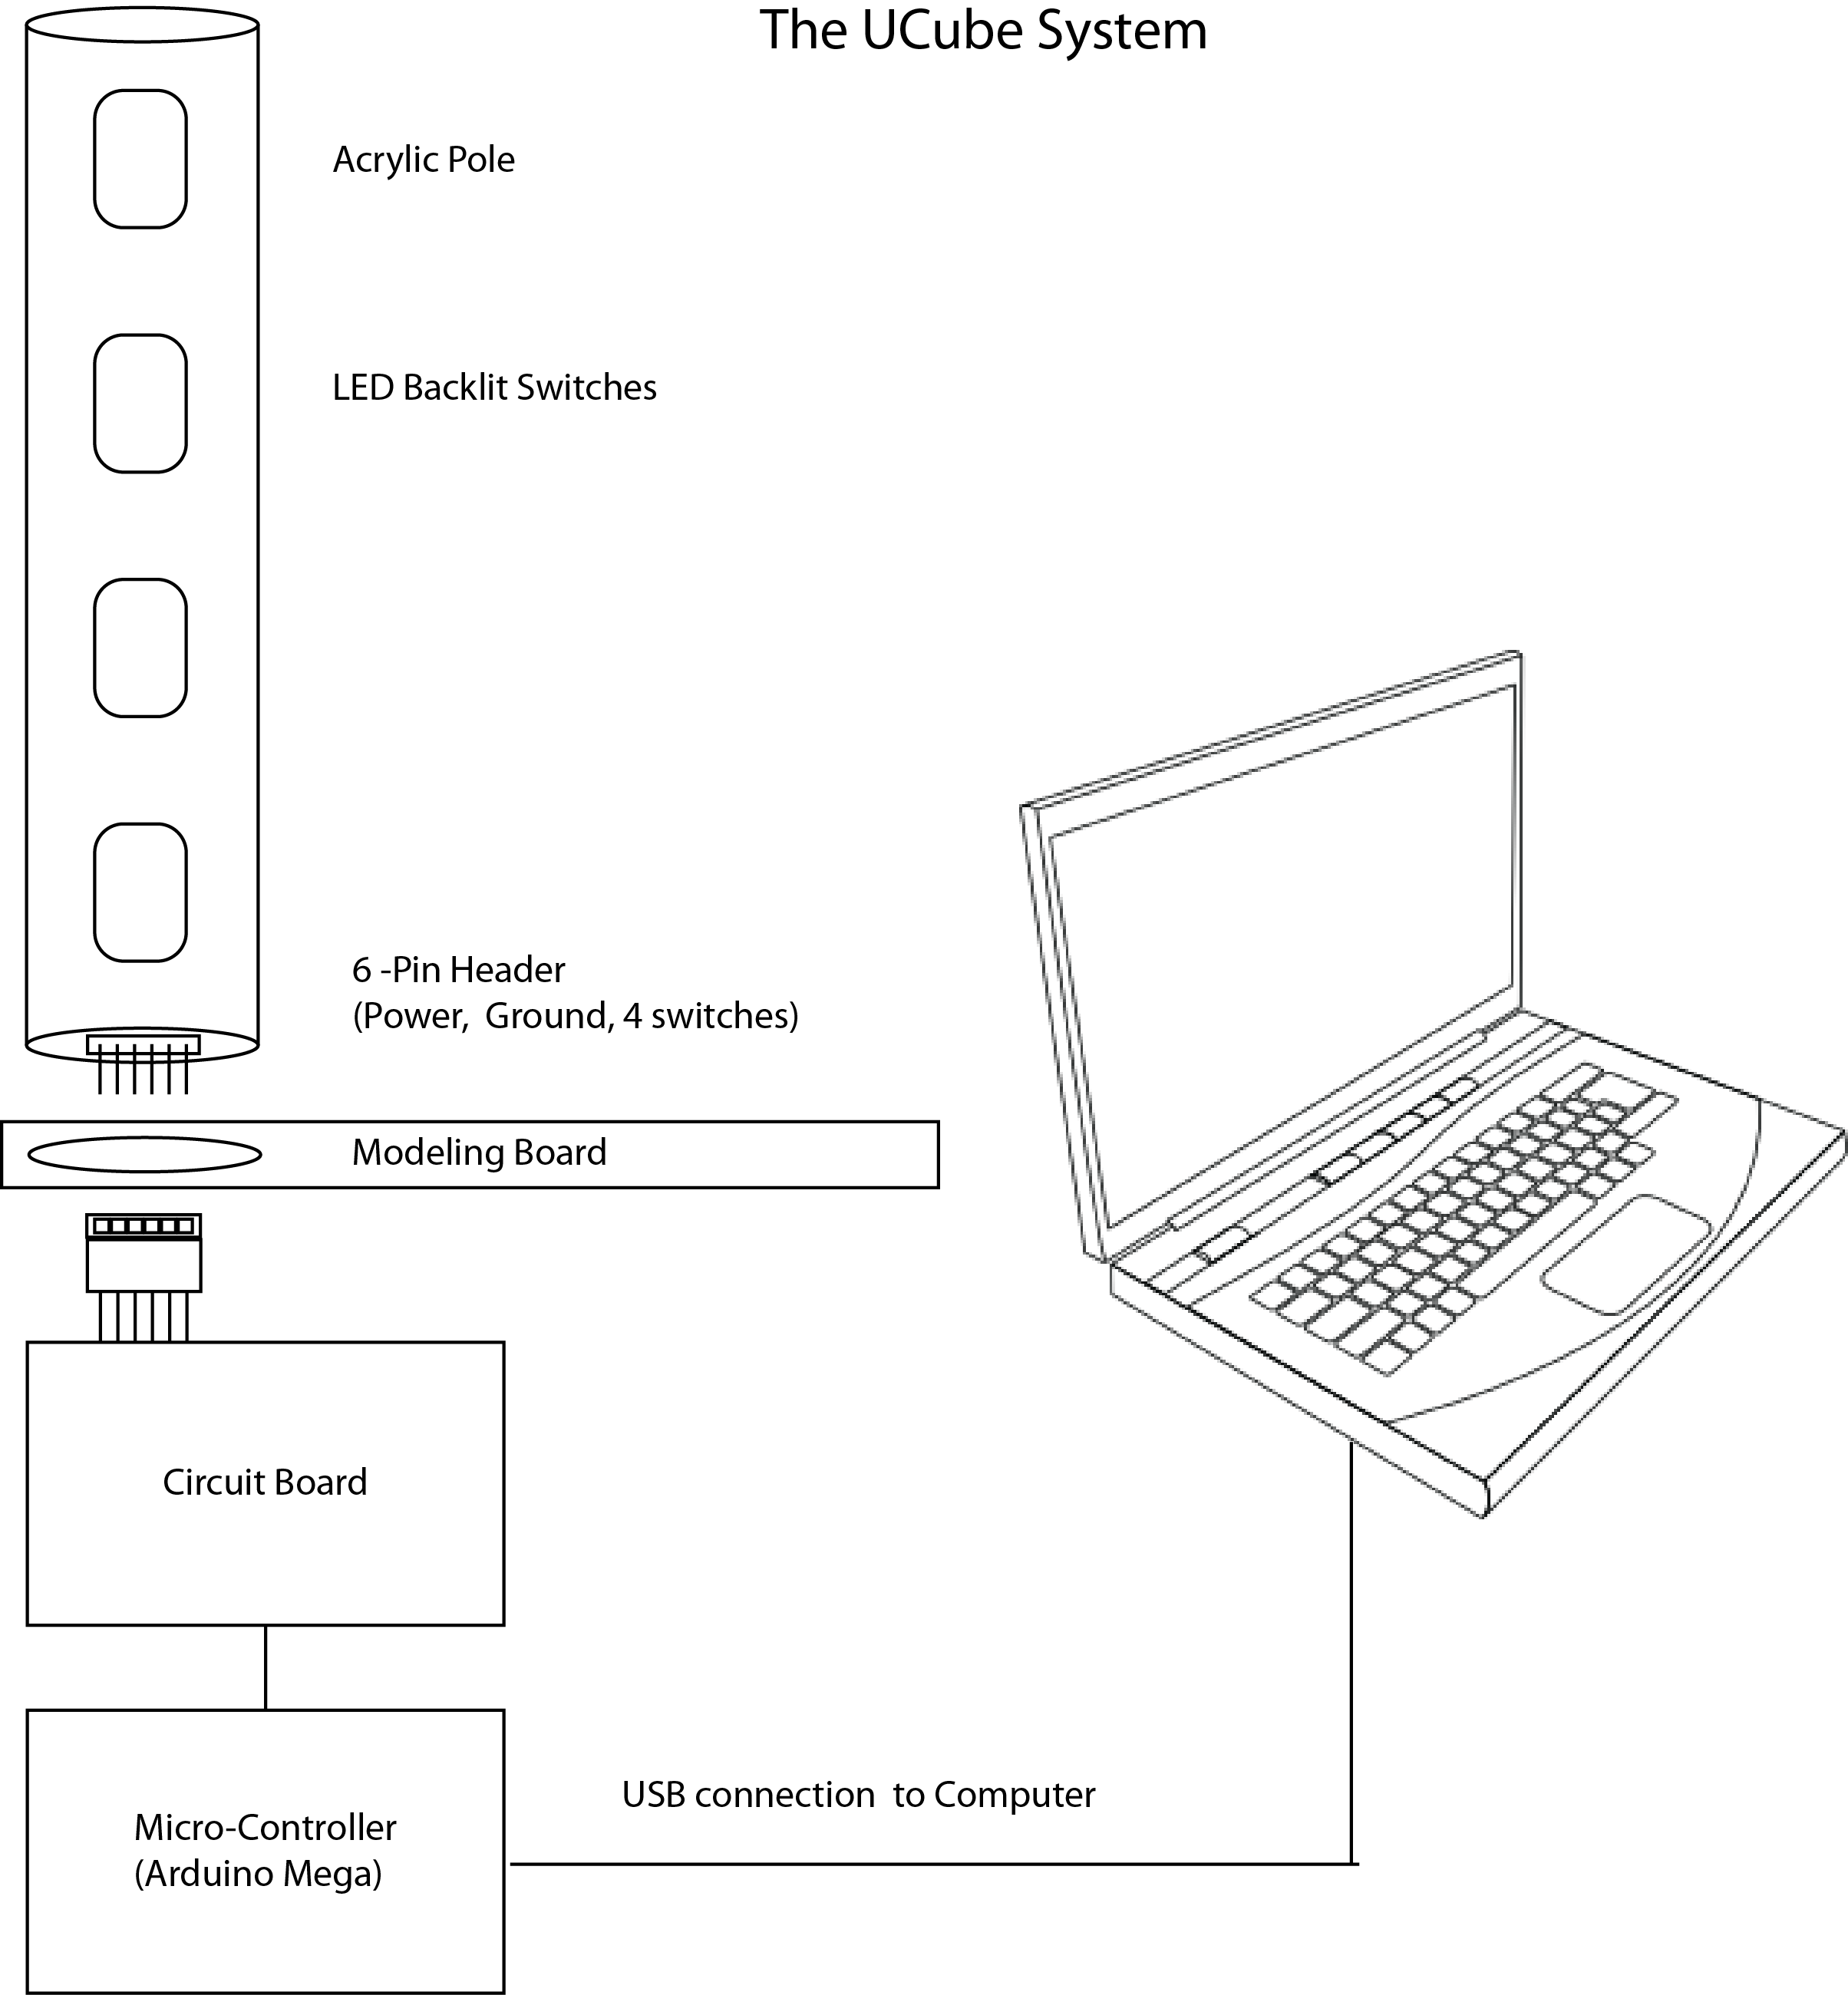
\includegraphics[width=.5\linewidth]{images/ucube_diagram}
\end{array}$
\end{center}
\caption{A schematic illustration of the UCube hardware.}
\label{fig:ucube1_schematic}
\end{figure}


% from IDC 2011 paper
As a first step in discussing the UCube's role in spatial design�and in
discussing the broader issue of children's three-dimensional design�this section
is devoted to a more thorough description of the UCube and its operation.
To begin with an overview, then: the UCube system is the combination of two
elements: the physical input device of ``towers'' placed on a board, and the
companion display software. These two systems work together to take the embodied
actions of the user and display corresponding points and shapes on the computer.
A sense of the scale of the device can be inferred from \ref{fig:cubev2}, which
shows a photograph of a middle-school student holding a newly-placed tower in
the UCube platform while pointing simultaneously at the desktop computer screen
beside it.
This photograph�which we will also return to in the discussion of pilot testing
in a later section�reflects the essential nature of interaction with the device:
points are designated in a spatial region provided by the platform, and then
represented in real time on the computer screen. Thus, the UCube promotes an
attention to the correspondence between the selected spatial points above the
platform and the (more abstract) representation on the computer screen.

\subsection{Technical Implementation} 
The physical system for our first UCube prototype, as outlined earlier, consists
of a platform with a four-by-four grid of potential sites, each of which can
hold one tower with four switches, thus describing a 4x4x4 array of 64 potential
points.
The platform structure consists of three different horizontal ``layers''. The
top (or upper surface) layer has a four-by-four grid of circular holes, into
which the towers fit snugly. This layer of 1/4'' thick laser-cut clear acrylic
acts as a brace to hold the towers upright, and ensures that they are resistant
to being knocked over. The next layer down holds the headers, which allow the
towers to ``plug in'' and connect to the rest of the circuit. Wires from the
headers go down to the bottom layer, which holds the breadboarded circuit and
Arduino Mega microcontroller. The towers are made of transparent acrylic, the
side paneling of basswood. The towers were laser-cut in order to house the four
switches and corresponding circuitry elements. The switches are LED-backlit when
active, making it more apparent which points are active as well as giving a more
accessible ``gestalt'' of the shape being modeled. It also allows for some
potentially interesting applications in dimly-lit circumstances, such as
modeling constellations in a classroom or planetarium: in these situations, the
lights of the selected spatial points stand out especially vividly.

Each tower connects to the platform through a six-pin header (one pin each for
power, ground, and four switches). The switch connections are then routed
through a breadboard containing current limiting resistors for the LED switches
to pins on a microcontroller (an Arduino Mega\cite{ArduinoMega}).
The Arduino is then able to communicate (via asynchronous serial communication)
the active switches (and corresponding coordinates) to the computer through a
USB cable. \ref{fig:ucube1_schematic} depicts a schematic diagram of the
UCube hardware.

\subsection{A Sample UCube Scenario}
As a sample scenario, imagine that we wish to create a triangular prism solid
employing the UCube. We can begin this process by selecting three points to form
a triangle, as shown in Figure 6; then, by placing two more towers and creating
the same triangular shape "shifted over" by two units (Figure 7) we create the
entire prism. Naturally, there might be many alternative pathways to forming the
same eventual shape: for example, we might begin by placing four (or more)
towers in the platform, and then experiment or fiddle with the chosen lights to
approach the eventual goal of creating our prism. Alternatively, we might begin
without any towers in the device at all: by placing our hands or fingers above
the device, roughly indicating where the prism should be, we might then use our
imagined locations as "guides", helping us to place the necessary towers in the
platform and select the correct lights for the vertices of the prism.
In any event, having designed the prism using the UCube platform, and having
checked that it looks like the correct shape on the computer screen, the final
step is to export the shape into a format suitable for 3D printer output. The
UCube software, as noted earlier, includes a feature for doing just this; and
finally, we print out the prism, as shown in Figure 8.
Figure 6. The first step in constructing our triangular prism: here, we create a
planar triangular shape toward the left side of the platform, and can see the
resulting shape on the computer screen shown at right.
Figure 7. Completing the triangular prism. Here, we have added a second
("shifted") version of our original triangle to produce the six vertices needed
to form the prism.

\subsection{Limitations}
It will probably not have escaped the reader's notice that the UCube, as a
three-dimensional modeling device, has significant limitations. To take the most
glaring of these: the user can only model those shapes whose vertices are among
the sixty-four locations accessible from the device. Moreover, those available
locations are evenly spaced in the form of a three-dimensional grid, or lattice;
thus, there are numerous simple-but-interesting shapes (such as the regular
dodecahedron, composed of regular pentagonal faces) that cannot be designed in
the current version of the UCube. Likewise, shapes with curved surfaces (such as
a cylinder), demanding at the very least a high resolution of accessible points,
could not be modeled in the current UCube. We will return to these issues in the
final section of the paper, in the discussion of ongoing and future work.



\section{SnapCAD}

Based on the feedback from these two user studies, a second, more powerful
instantiation of the ideas from the UCube has been created. SnapCAD (formerly
known as UCube v2) consists of a total input space of 7x7x7 points, forming 343
distinct coordinates. In our user studies with UCube v1, we noticed that users
often encountered initial difficulties when required to ``find a middle'' in the
shape they were attempting to model, given an even number of total grid spaces.
For example, to model a pyramid on on a 4x4x4 grid, one needs to construct a 3x3
subset of the 4x4 grid, using the middle point within the 3x3 set as the top of
the pyramid. This influenced our decision to create an odd-numbered layout,
creating a more ``natural'' middle point in the hardware. The greater number of
inputs vastly increases the expressive potential of SnapCAD (compared to the
UCube) while still maintaining a manageable interface. SnapCAD, as seen in
\ref{fig:snap1} has some very obvious differences from its predecessor.

\begin{figure}[ht] \begin{center}$
\begin{array}{cc}
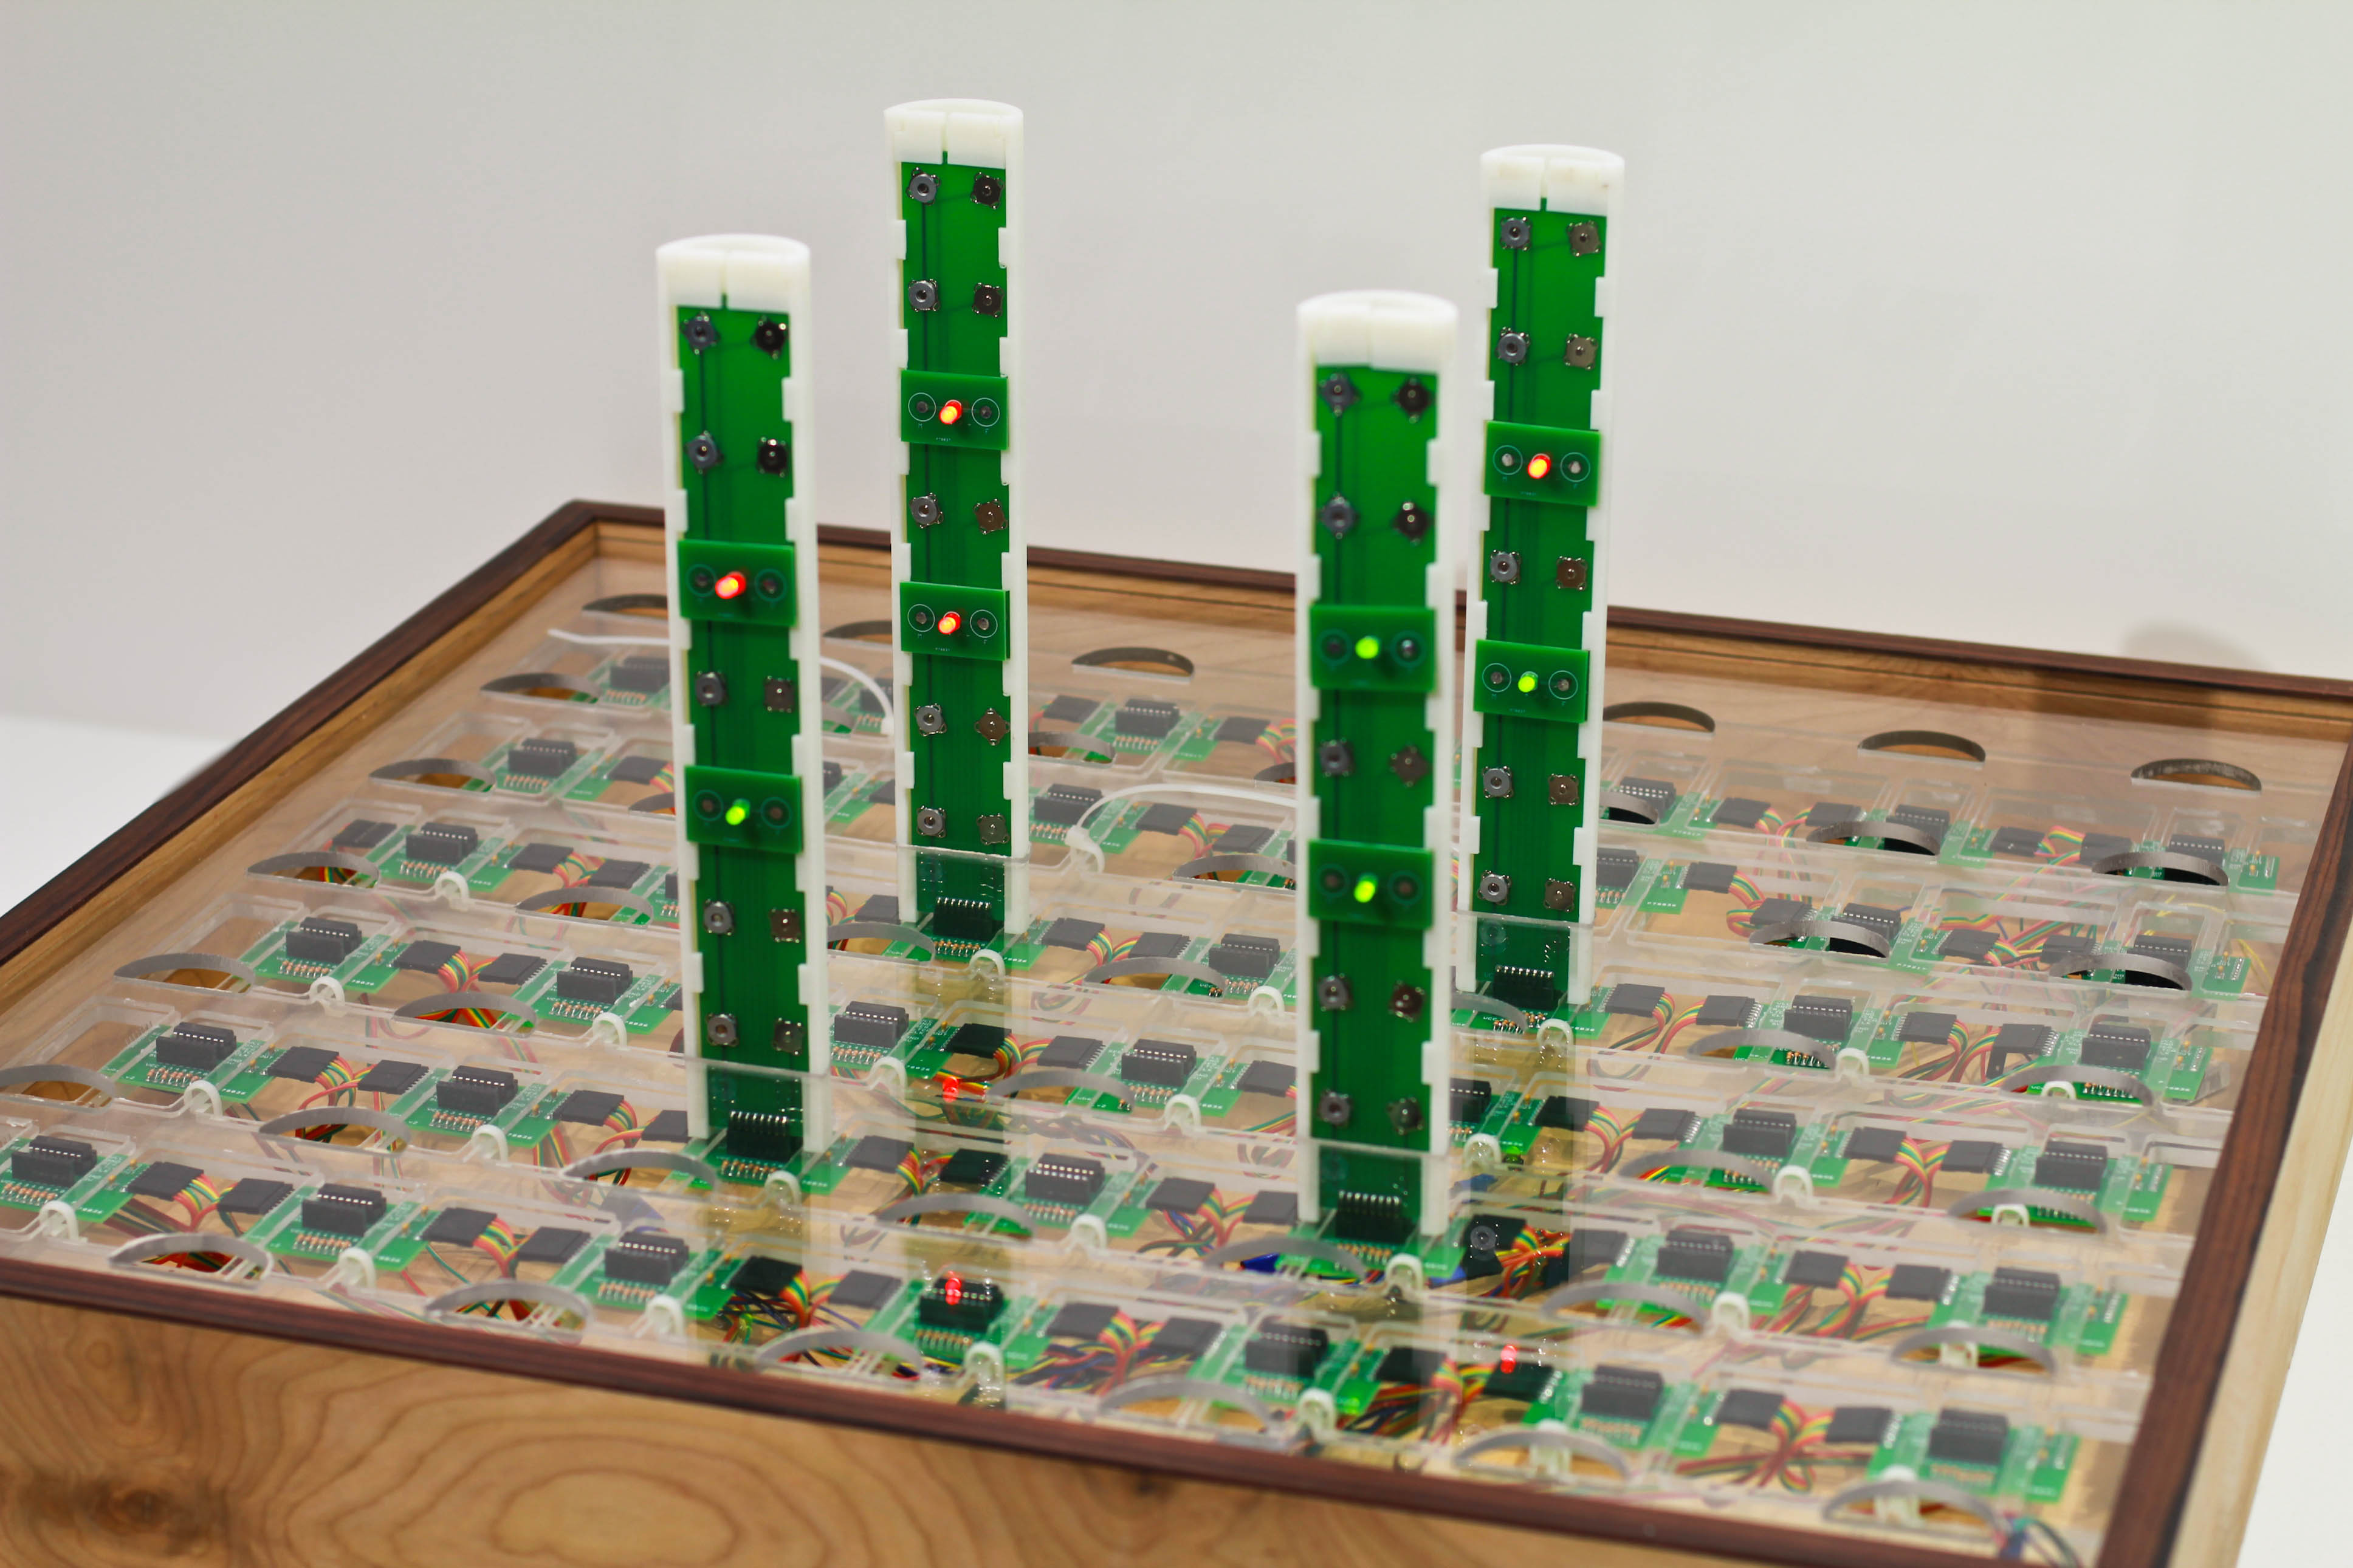
\includegraphics[width=.45\linewidth]{images/BeatriceFinal-2}& 
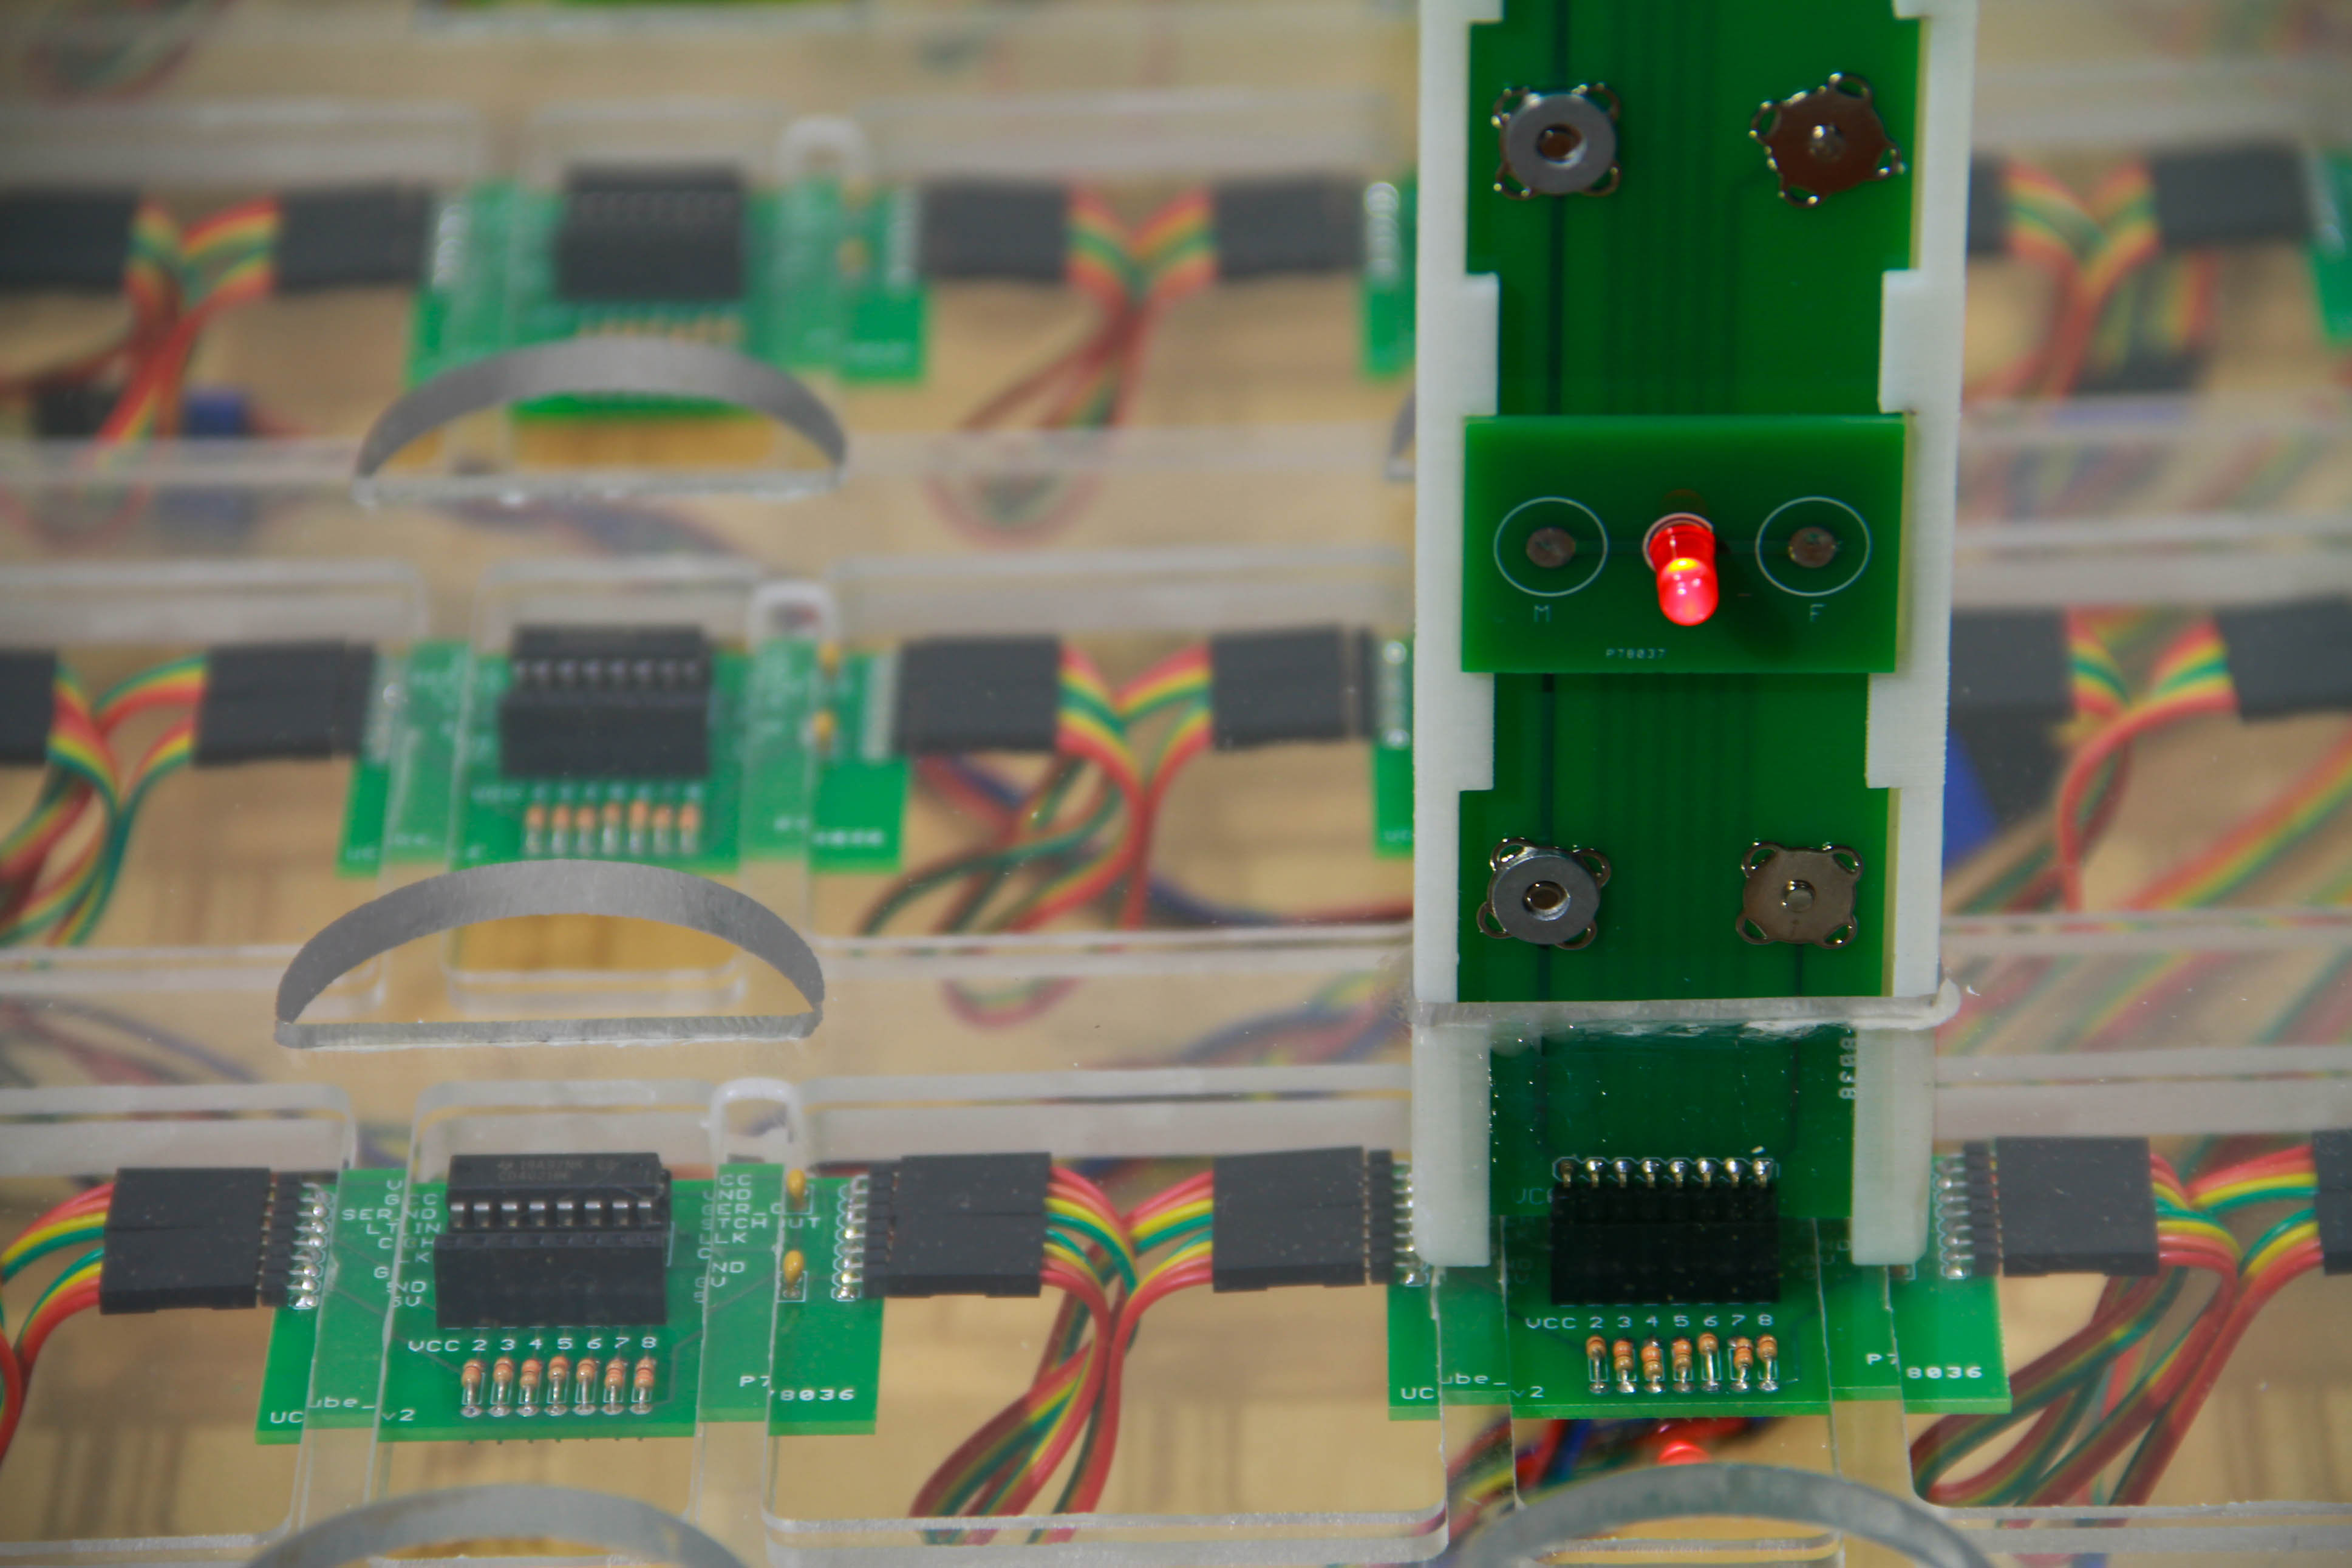
\includegraphics[width=.45\linewidth]{images/BeatriceFinal-14}
\end{array}$
\end{center}
\caption{
Left: the SnapCAD interface, showing the hardware configuration corresponding to
the picture below in \ref{fig:snap2}. Right: a detail of the SnapCAD
hardware - the PCB tower is housed in a 3D-printed shell, which plugs into a
shift-register board. The LED boards snap on to the towers via magnetic snaps.}
\label{fig:snap1}
\end{figure}

Working on the scale of multiple hundreds of inputs necessitated the design of
custom circuit boards to relay information effectively to the microcontroller.
This change in scale also meant rewriting most of the modeling software to
effectively handle the greater expressiveness of the physical system.



\begin{figure}[ht] \begin{center}$
\begin{array}{cc}
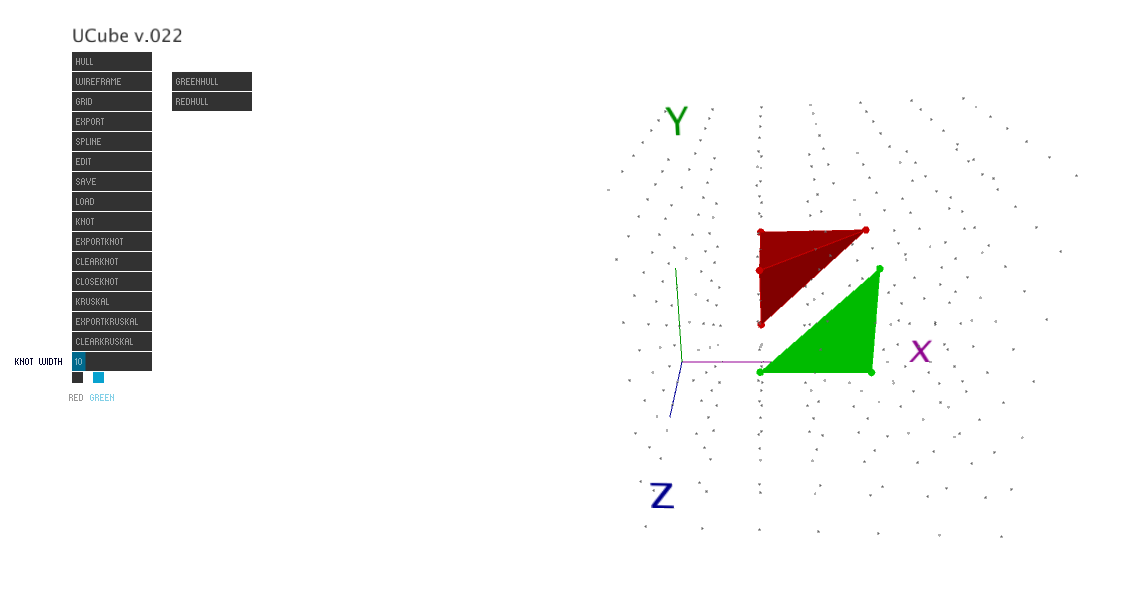
\includegraphics[width=.45\linewidth]{images/twoHulls} &
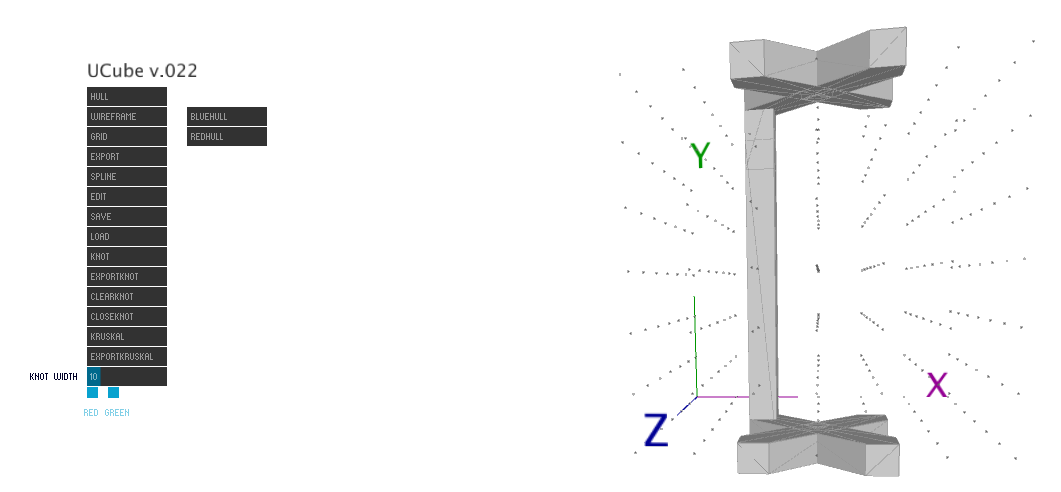
\includegraphics[width=.45\linewidth]{images/mst}
\end{array}$
\end{center}
\caption{Left: The SnapCAD software showing two convex hulls of different
colors. Right: the SnapCAD software showing a minimal spanning tree model.}
\label{fig:snap2}
\end{figure}


The use of conductive, magnetic snaps along towers constructed of custom-printed
circuit board allow for more than one color of illumination, as different
colored LED boards can be snapped onto any socket on the tower.
This not only results in the ability to represent multiple shapes at once, but
for the SnapCAD to become a platform for all manner of multi-player interactions
(e.g. games, puzzles, shape matching contests), with each ``player'' assigned a
unique color. To this end, we have created a simple ``3D Tic-Tac-Toe''
implementation on the SnapCAD. Additional changes to the software include
supporting multiple but separate convex hulls of different colors, the ability
to create and export shapes created from the minimal spanning tree of a set of
input points, and the ability to adjust the width of the segments in the
knot/path and minimal spanning tree modes.
The click-and-drag editing mode now includes the knot/sequential path and
minimal spanning tree modes as well as the convex hull mode. We also adjusted
the knot-forming algorithm to handle paths that cross or self-intersect, as well
as providing a ``close knot'' button to complete a circuit in a shape, allowing
for even more kinds of 3D-printable objects. While significant work has been
done to bring the UCube and SnapCAD to their current states, we believe not only
that there is room for additional improvements to be made, but that, as opposed
to focusing on a incremental but essentially similar interface as the subject of
a thesis, it is far more intellectually interesting to focus on a class of
objects that demonstrate multiple incarnations of a set of ideas.

\begin{figure}[!ht] 
\begin{center}$
\begin{array}{cc}
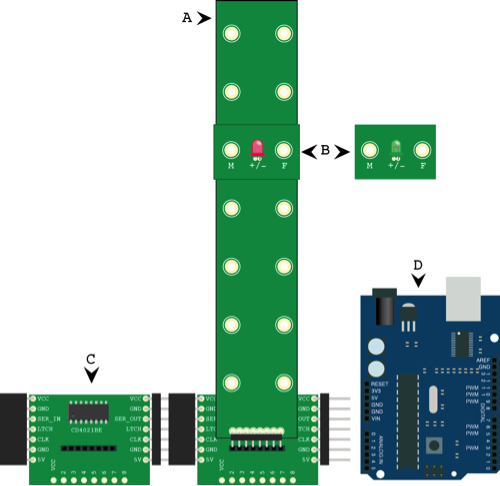
\includegraphics[width=.45\linewidth]{images/snap_schematic}
\end{array}$
\end{center}
\caption{A schematic of the SnapCAD technical design, showing a sample tower
(A), LED light element (B), shift register board (C) and Arduino (D). The Arduino
microcontroller's role is to send coordinates (and colors) of the LED lights,
once placed, to a desktop computer. A fuller description of this schematic is
provided in the accompanying text.}
\label{fig:snap3}
\end{figure}

\subsection{A Sample (Red/Green Player) Strategy Game for SnapCAD}

Each of the previous
sample projects could have been undertaken with the UCube 1.0 (although in every
case, the larger scale of the UCube 2.0 allows for a far greater quantitative
range of construction�for example, one can create polyhedra or paths in a
7-by-7-by-7 grid that would be impossible in a 4-by-4-by-4 grid). In this last
example, we will make use of the two-color capability of the UCube to suggest a
hypothetical game, or genre of game, that could be created with the system.
The imagined game in question is a geometric strategy game between two players,
"Red" and "Green". At the outset of the game, each player is given four lights
of her own color; the two of them are told to place their lights at the eight
corners of a cube in the positions shown in the photograph shown in Figure 9.
Now, the computer could display the convex hull of the present set of lights (a
cube), as shown in Figure 10; and then (in our scenario) the computer tells the
Green player to move one of her lights to create the new convex hull shown at
the right of Figure 10. Thus, the Green player's job is to change the "cube"
hull to the new hull with one move of one green light. A correct answer to this
challenge is shown in the photograph of Figure 11; and if the Green player makes
this correct move, the Red player is now given the (current) convex hull and yet
another hull that could be created with one move of a red light. In this
fashion, the two players take turns moving lights of their own color to produce
a new overall configuration of lights at every step, until one player fails to
solve the current challenge, at which point the game is over.
There are, of course, many variants or extensions of this game that could be
imagined (for instance, a player might be asked to shift two lights, or to add a
new additional light in her color, to create a new convex hull). The purpose of
this example is simply to show that, with the inclusion of two available colors
for spatial points in UCube 2.0, a sizeable potential landscape of geometric
activities and puzzles becomes feasible.



% \section{Proposed Work: Technical Additions}
% The proposed work is in two sections: technical additions and
% evaluation. This section deals with the technical additions to the proposed
% devices: SnapCAD and PopCAD.
% 
% \subsection{SnapCAD}
% 
% With 343 potential points, a click-and-drag editing tool, and three separate
% modeling modes (convex hull, knot/path, and minimal spanning tree) the SnapCAD
% is capable of generating countless 3-dimensional forms.
% Although the potential for additional modeling tools is certainly a possibility
% (we have yet to experiment with curved surfaces, for instance) we believe that
% the multi-player `platform' aspects of the SnapCAD system are the most ripe for
% development. We already have two colors of LED boards, the ability to display
% two colors of convex hulls, and a 3D implementation of a two-player tic-tac-toe
% game. Displaying multiple colors of the path/knot and minimal spanning tree
% modes should be fairly straightforward to implement.
% We would also like to expand and change the colors currently being used - we
% currently use red and green LEDs, which would be problematic for anyone with
% red/green color blindness. We propose using three colors: red, blue, and purple.
% This not only allows for up to three-player interactions, but could help to
% solve a deeper problem: representing in hardware a node occupied by two players.
% Using an idiom where solely-occupied nodes are either blue or red, and a jointly
% occupied node is purple, we can then expand the types of games, puzzles, or
% modeling activities the SnapCAD system can support. Once these improvements are
% made we can expand the activities supported on SnapCAD. Developments include
% two-to-three player games like tic-tac-toe as well as games built
% off of the modeling capabilities of the SnapCAD (e.g. match the model generated
% by the computer, model a sequential path through a generated maze, place points
% on or interior to the convex hull until there are no more to be found). Colors
% can also be used for certain as-yet unexplored modeling operations (e.g., the
% set union, intersection, or difference). While some of these operations may
% prove difficult or even impossible, these are all avenues worth exploring, as
% they all point towards the extensibility and potential expressiveness of SnapCAD
% as a platform for future development.

\section{PopCAD}

Our motivations for creating alternative interfaces to the UCube and SnapCAD
stem from the desire to explore this intellectual space more generally; it is
far more interesting to discuss a \emph{class} of tangible interfaces for
scaffolding digital fabrication than it is to discuss a singular device. To this
end, we looked at some of the weaknesses of SnapCAD and towards technologies we
had yet to explore. While SnapCAD can admirably perform a number of modeling
tasks, it was always envisioned as one device amongst an `ecosystem' of next
generation fabrication tools. It has strengths, but obvious weaknesses as well;
in particular, the SnapCAD hardware was expensive to produce, and so would be a
difficult proposition for some schools or fab labs; it is also rather unwieldy
and unportable - it moderately heavy, fairly large, and has many separate pieces
that could break or go missing. Thus, an interface with cheaper and more
portable materials was desirable.

To address these issues we chose to build a pop-up book combining traditional
paper-crafts and paper-friendly electronics such as copper tape.
In recent years, revolutionary work has been done in combining electronics and
paper
crafting\cite{Qi:2010:EPE:1709886.1709909}\cite{Mellis:2013:MMC:2460625.2460638},
leading to new techniques and new uses for traditional materials. Paper is
inexpensive (especially when compared to circuit boards), light, and easily
portable, making it an ideal material choice for a device that would not suffer
the same limitations present in the SnapCAD. Although we often think of `paper'
as a rather static material, there are in fact many variations in the size,
weight, color, transparency, and composition of contemporary paper products. 

We will cover the two paper-based prototypes we created in this vein, dubbed
``PopCAD v1'' and ``PopCAD v2''.

\subsection{PopCAD v1}
For the initial prototype, we used a simple construction paper as it provided a
balance between strength and flexibility as well as having a consistency
well-suited to laser etching and cutting.
The pop-up book (named PopCAD) has a 3x3x3 array of 27 points which are evenly
spaced 3 inches apart on a 12'' x 18'' paper surface.
The book folds on a single center crease making the closed footprint of the book
roughly 12'' x 9''.

\begin{figure}[!ht] \begin{center}$
\begin{array}{cc}
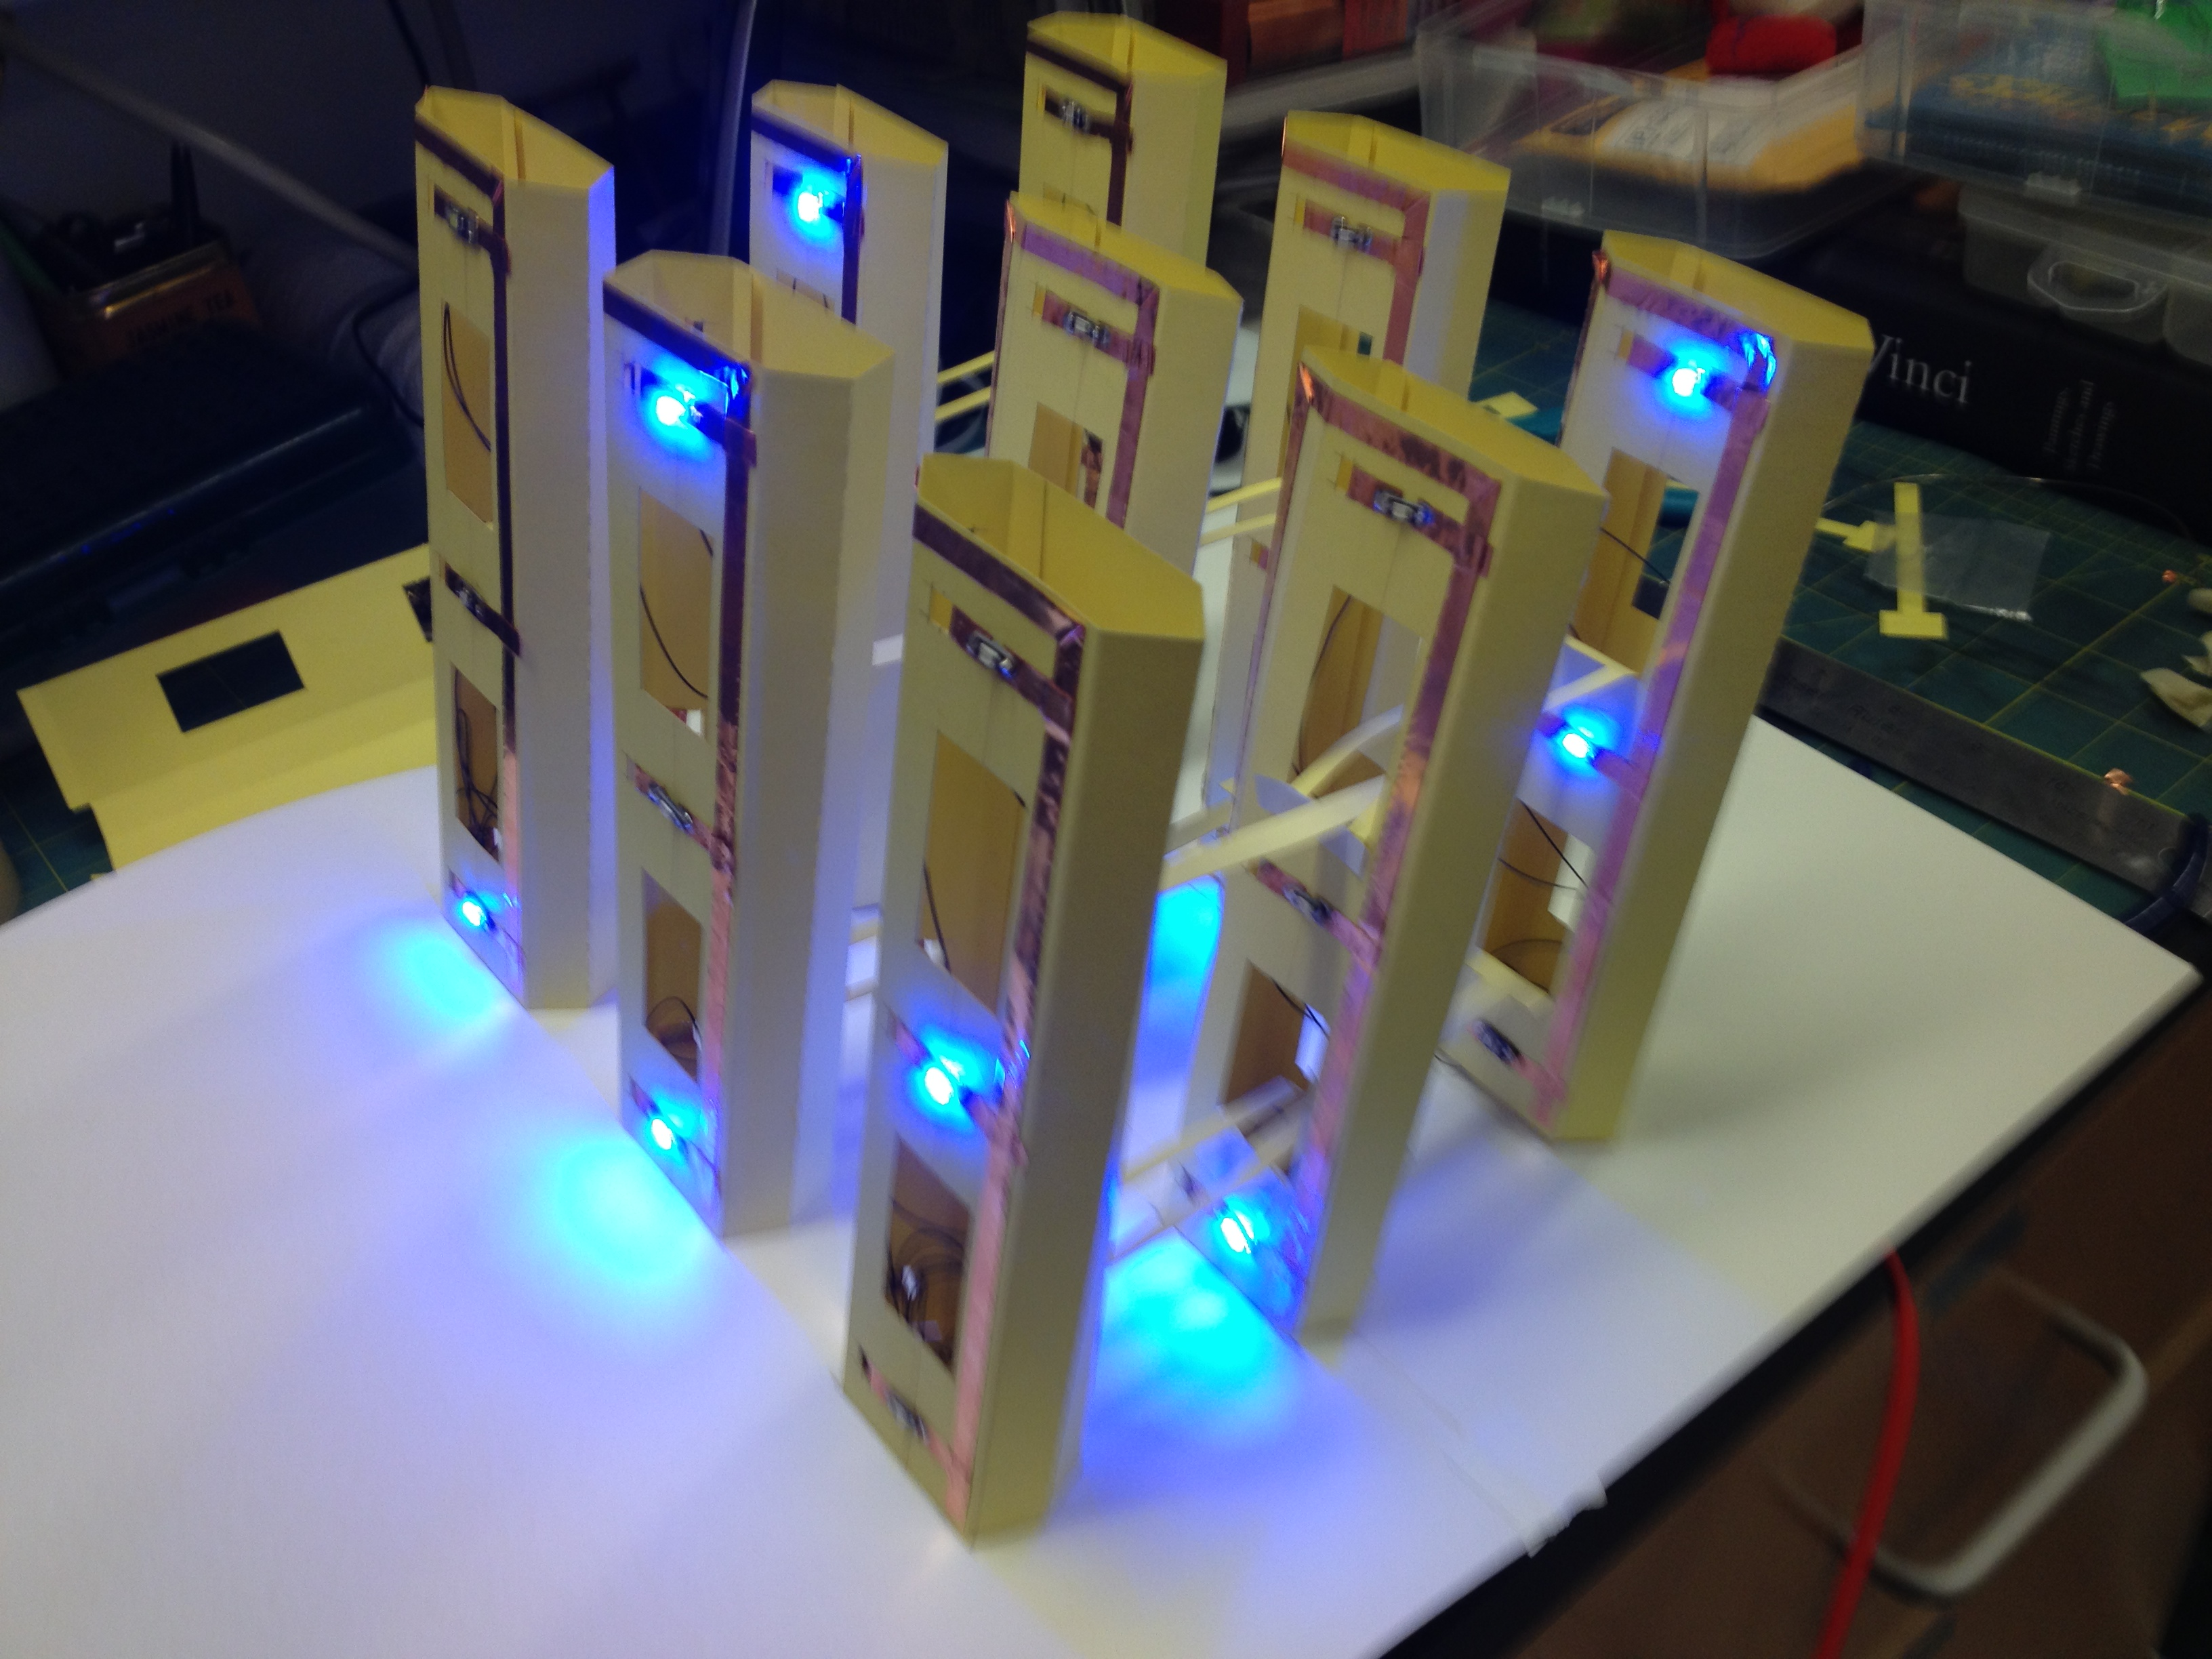
\includegraphics[width=.45\linewidth]{images/popup1}&
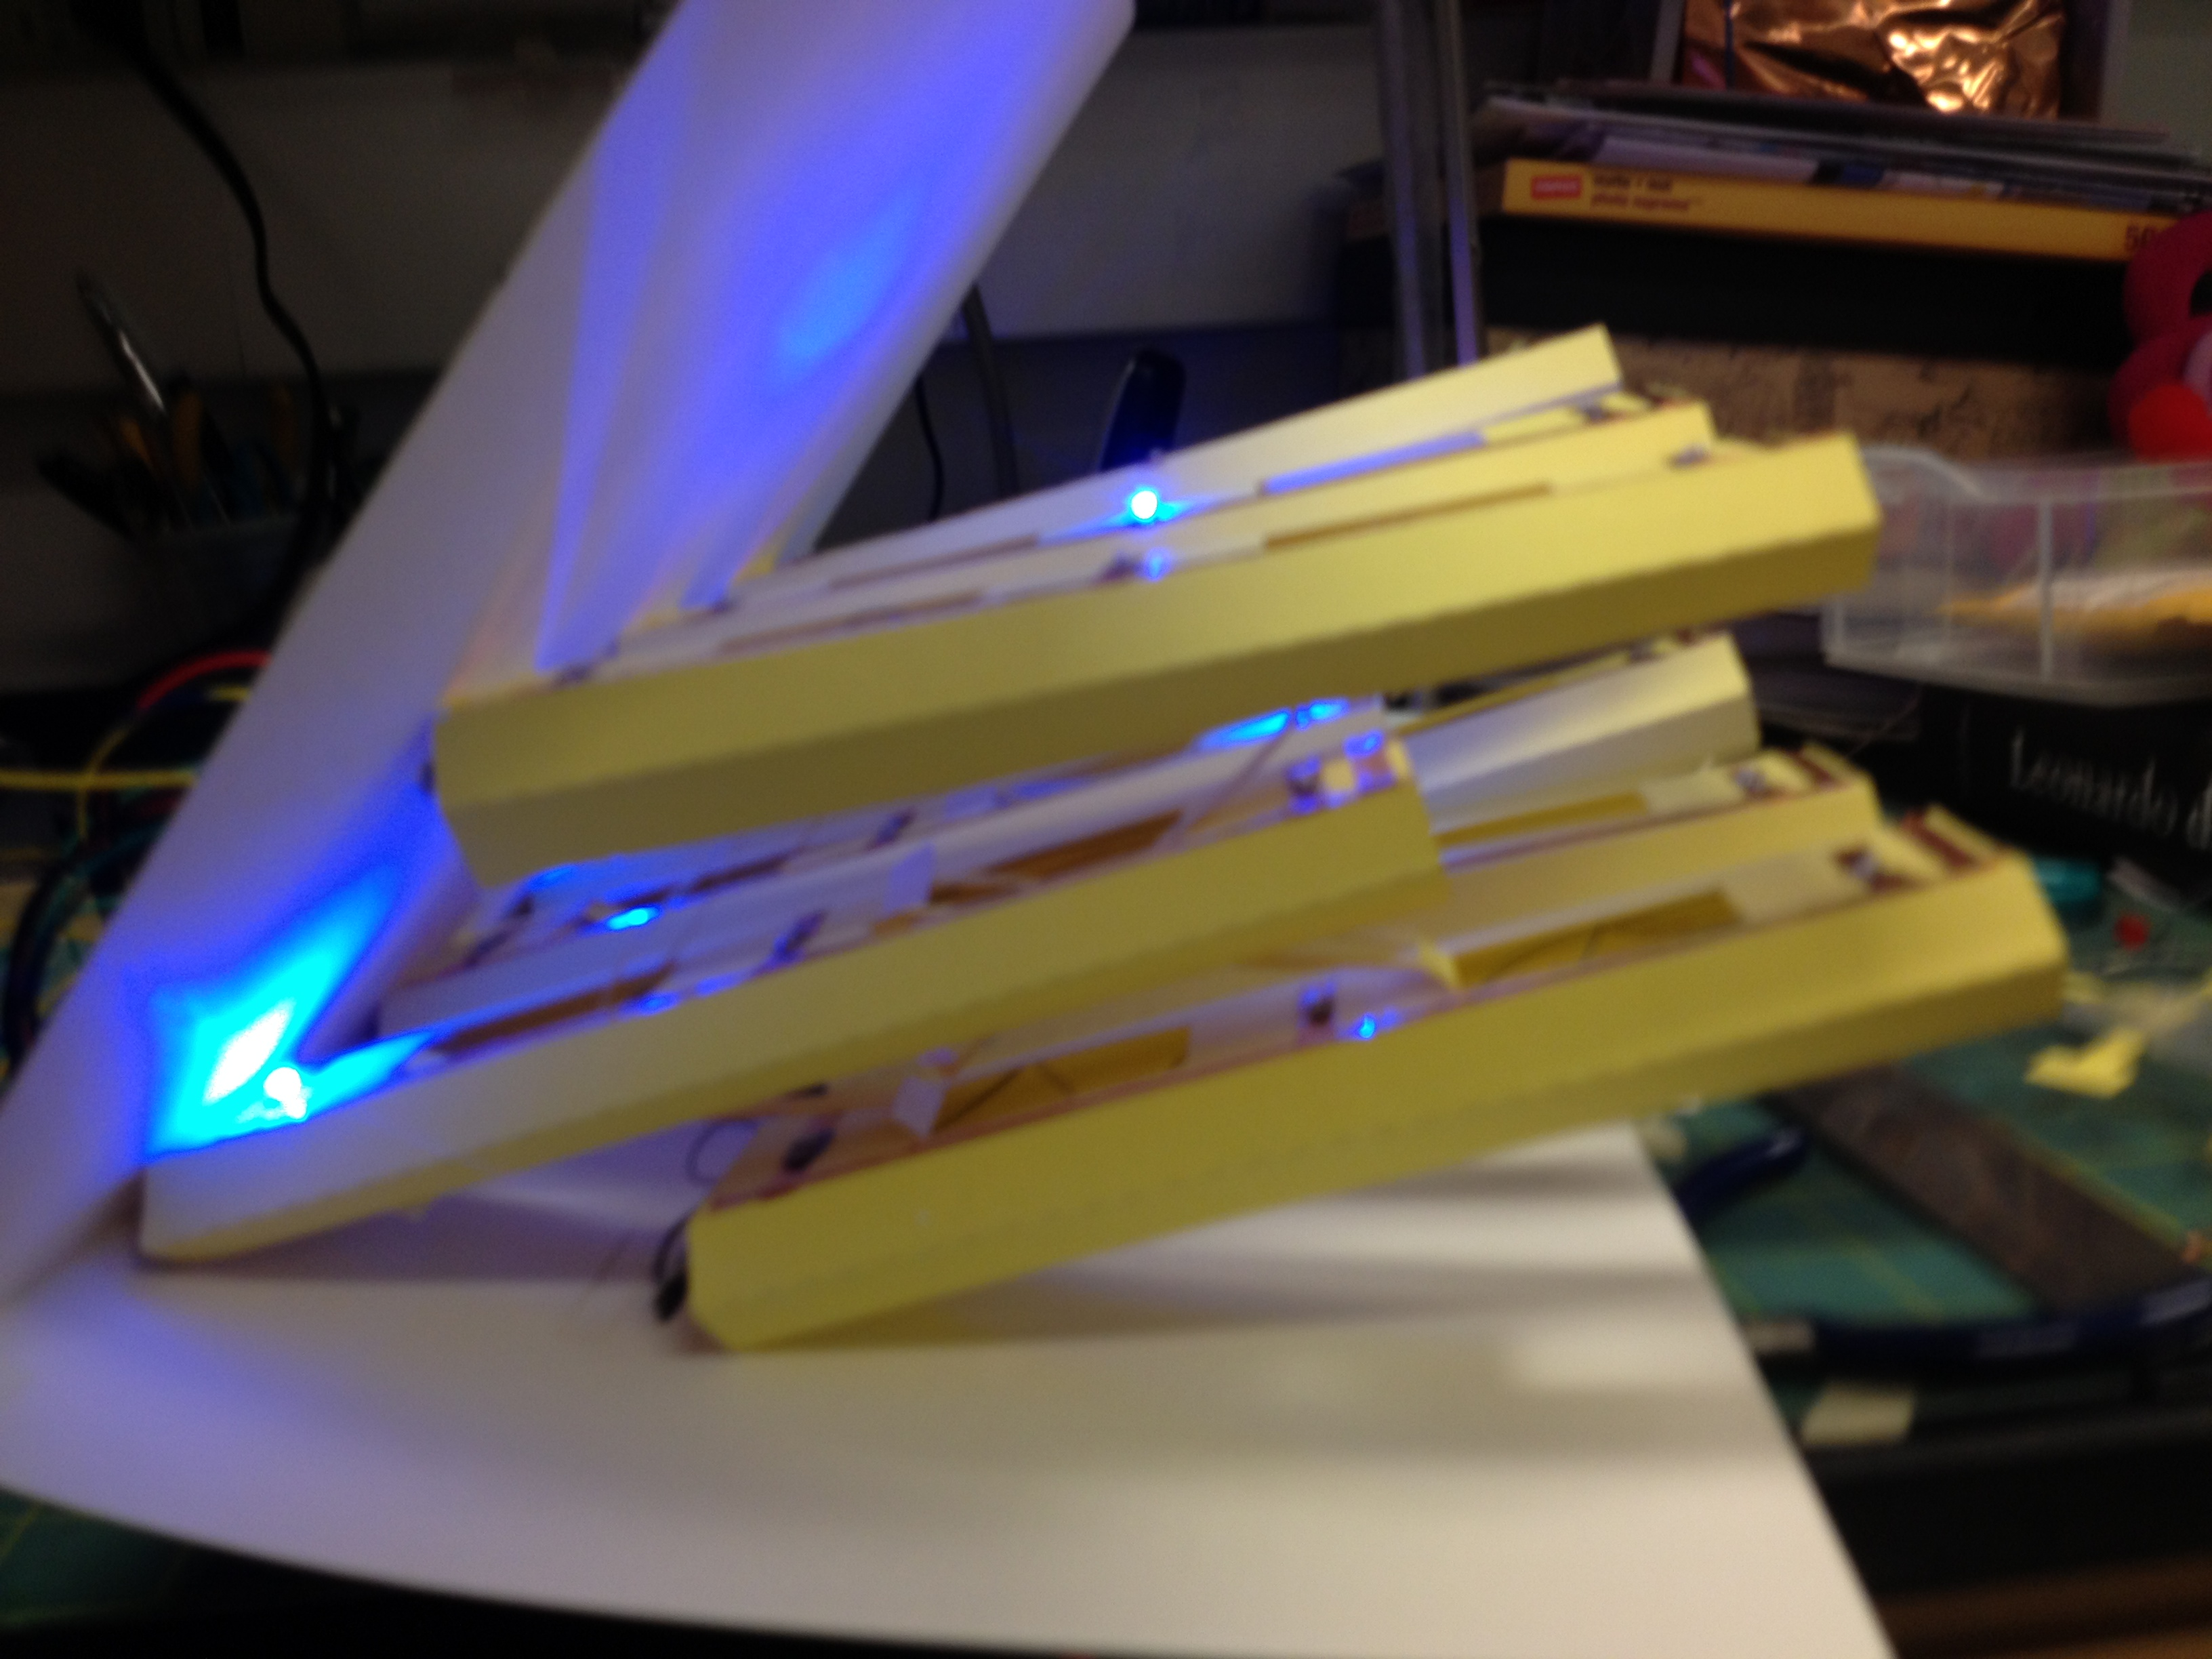
\includegraphics[width=.45\linewidth]{images/popup2}
\end{array}$
\end{center}
\caption{Two views of the pop-up book prototype, showing the paper towers and 
LEDs in both open and closed states.}
\label{fig:popup}
\end{figure}

Each tower has a copper tape circuit consisting of three LEDs on the front face
and three corresponding capacitive touch sensors on the left face. The copper
tape acts as a paper-friendly conductive material to connect the electronic
components together much like traditional wire. The LEDs are soldered onto the
copper tape for greater stability. The capacitive sensors are simply a piece of
copper tape which is connected to a pin on a microcontroller (in the first
version, this is an Arduino Mega Pro). By bringing the internal pull-up resistor
connected to the pin ``LOW'' (to ground) and then timing how long it takes to get
back to a ``HIGH'' state we can tell if the connection is being influenced by a
capacitive force. For example, if there is no interference on the circuit, the
timer will normally only get to ``1'' before the resistor is back to a HIGH state;
if a finger is placed on the copper tape, the reading will be
much higher (typically around ``17''). Based on this change, we can detect which
switch was touched and toggle the associated LED on or off. The hollow interior
of each paper tower is used to solder thin 30-gauge wire to the three LEDs, the
three switches, and ground. These seven wires are soldered to a row of headers
that stick through the bottom of the first layer of the pop-up book. Wires are
then run along the backside of the top layer of paper from these headers to the
microcontroller. The entire circuit in then encased in a cloth-covered cardboard
binder that acts as a book cover as well as a means to protect and hide the
electronics.

\begin{figure}[!ht] \begin{center}$
\begin{array}{cc}
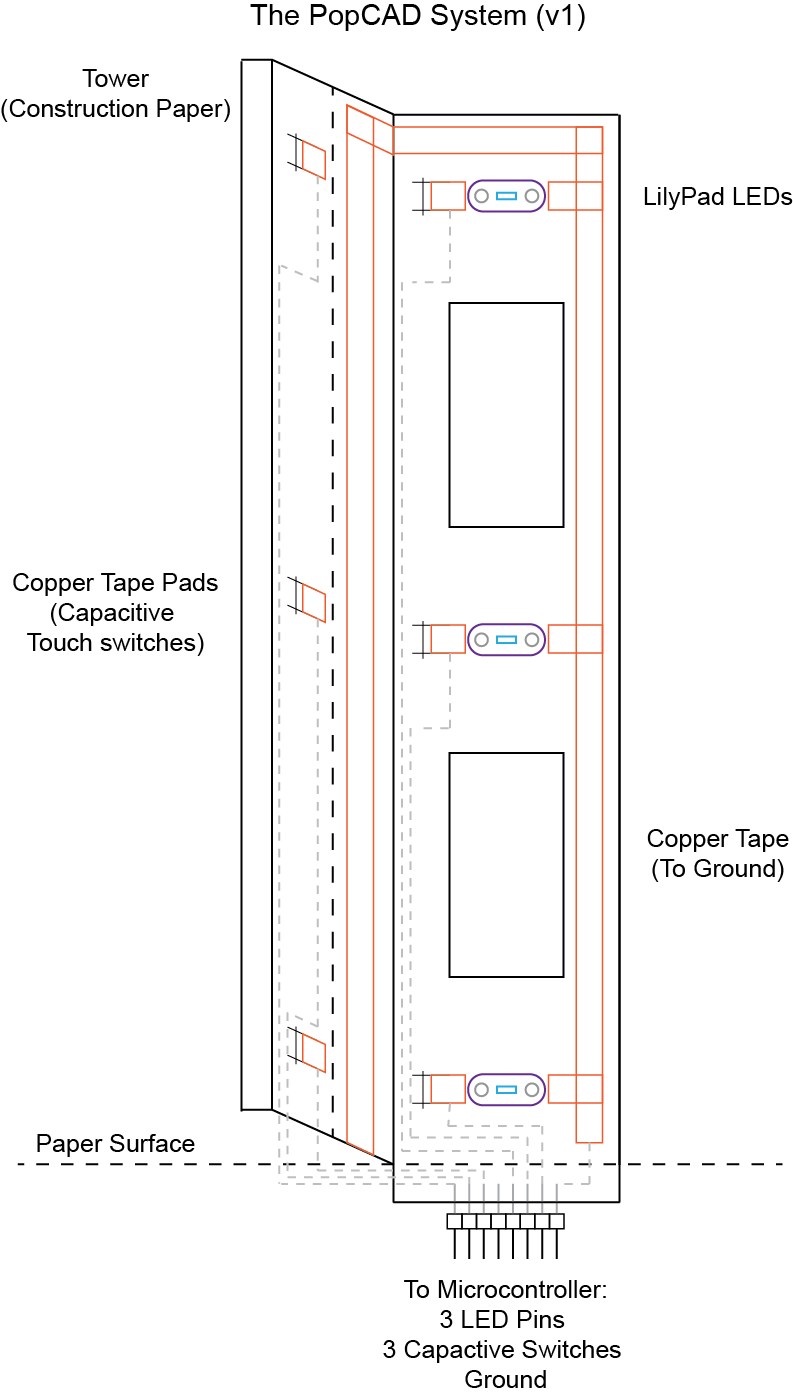
\includegraphics[width=.4\linewidth]{images/PopCadSchematicV1}&
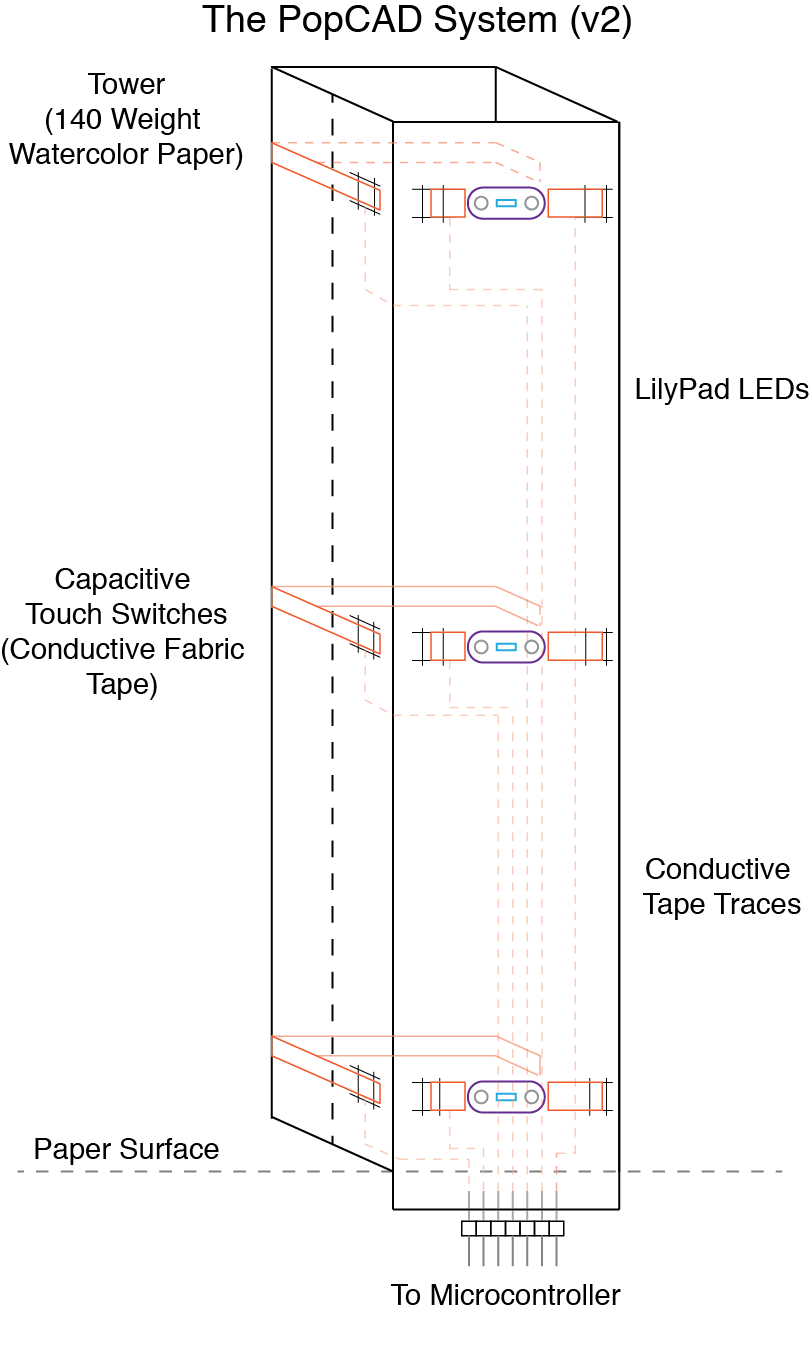
\includegraphics[width=.42\linewidth]{images/PopCadSchematicV2}
\end{array}$
\end{center}
\caption{The two PopCAD designs side-by-side: PopCAD v1 (left) uses copper tape
and 30 gauge wire for the paper circuit, while PopCAD v2 (right) uses
fabric-based conductive tape without needing any wires.}
\label{fig:popup_schematic1}
\end{figure}

\subsection{PopCAD v2}

This is where we talk about the differences: conductive tape, laser cutting,
paper choice circuit wiring is more efficient, no horizontal struts\ldots

Although the first PopCAD iteration was a fully-functional prototype, as we
approached evaluating the PopCAD in user testing it became apparent that there
were several compelling reasons to iterate on the original design. Through a few
informal user evaluations as well as our own reflections on the device, we
identified several key issues that could be improved upon: (a) the paper
engineering design, (b) the structural integrity of the book as a whole, and (c)
the lack of ``paper-ness'' with respect to the circuitry and electrical
components of the design.

 \begin{figure}[!ht]
  \centering
  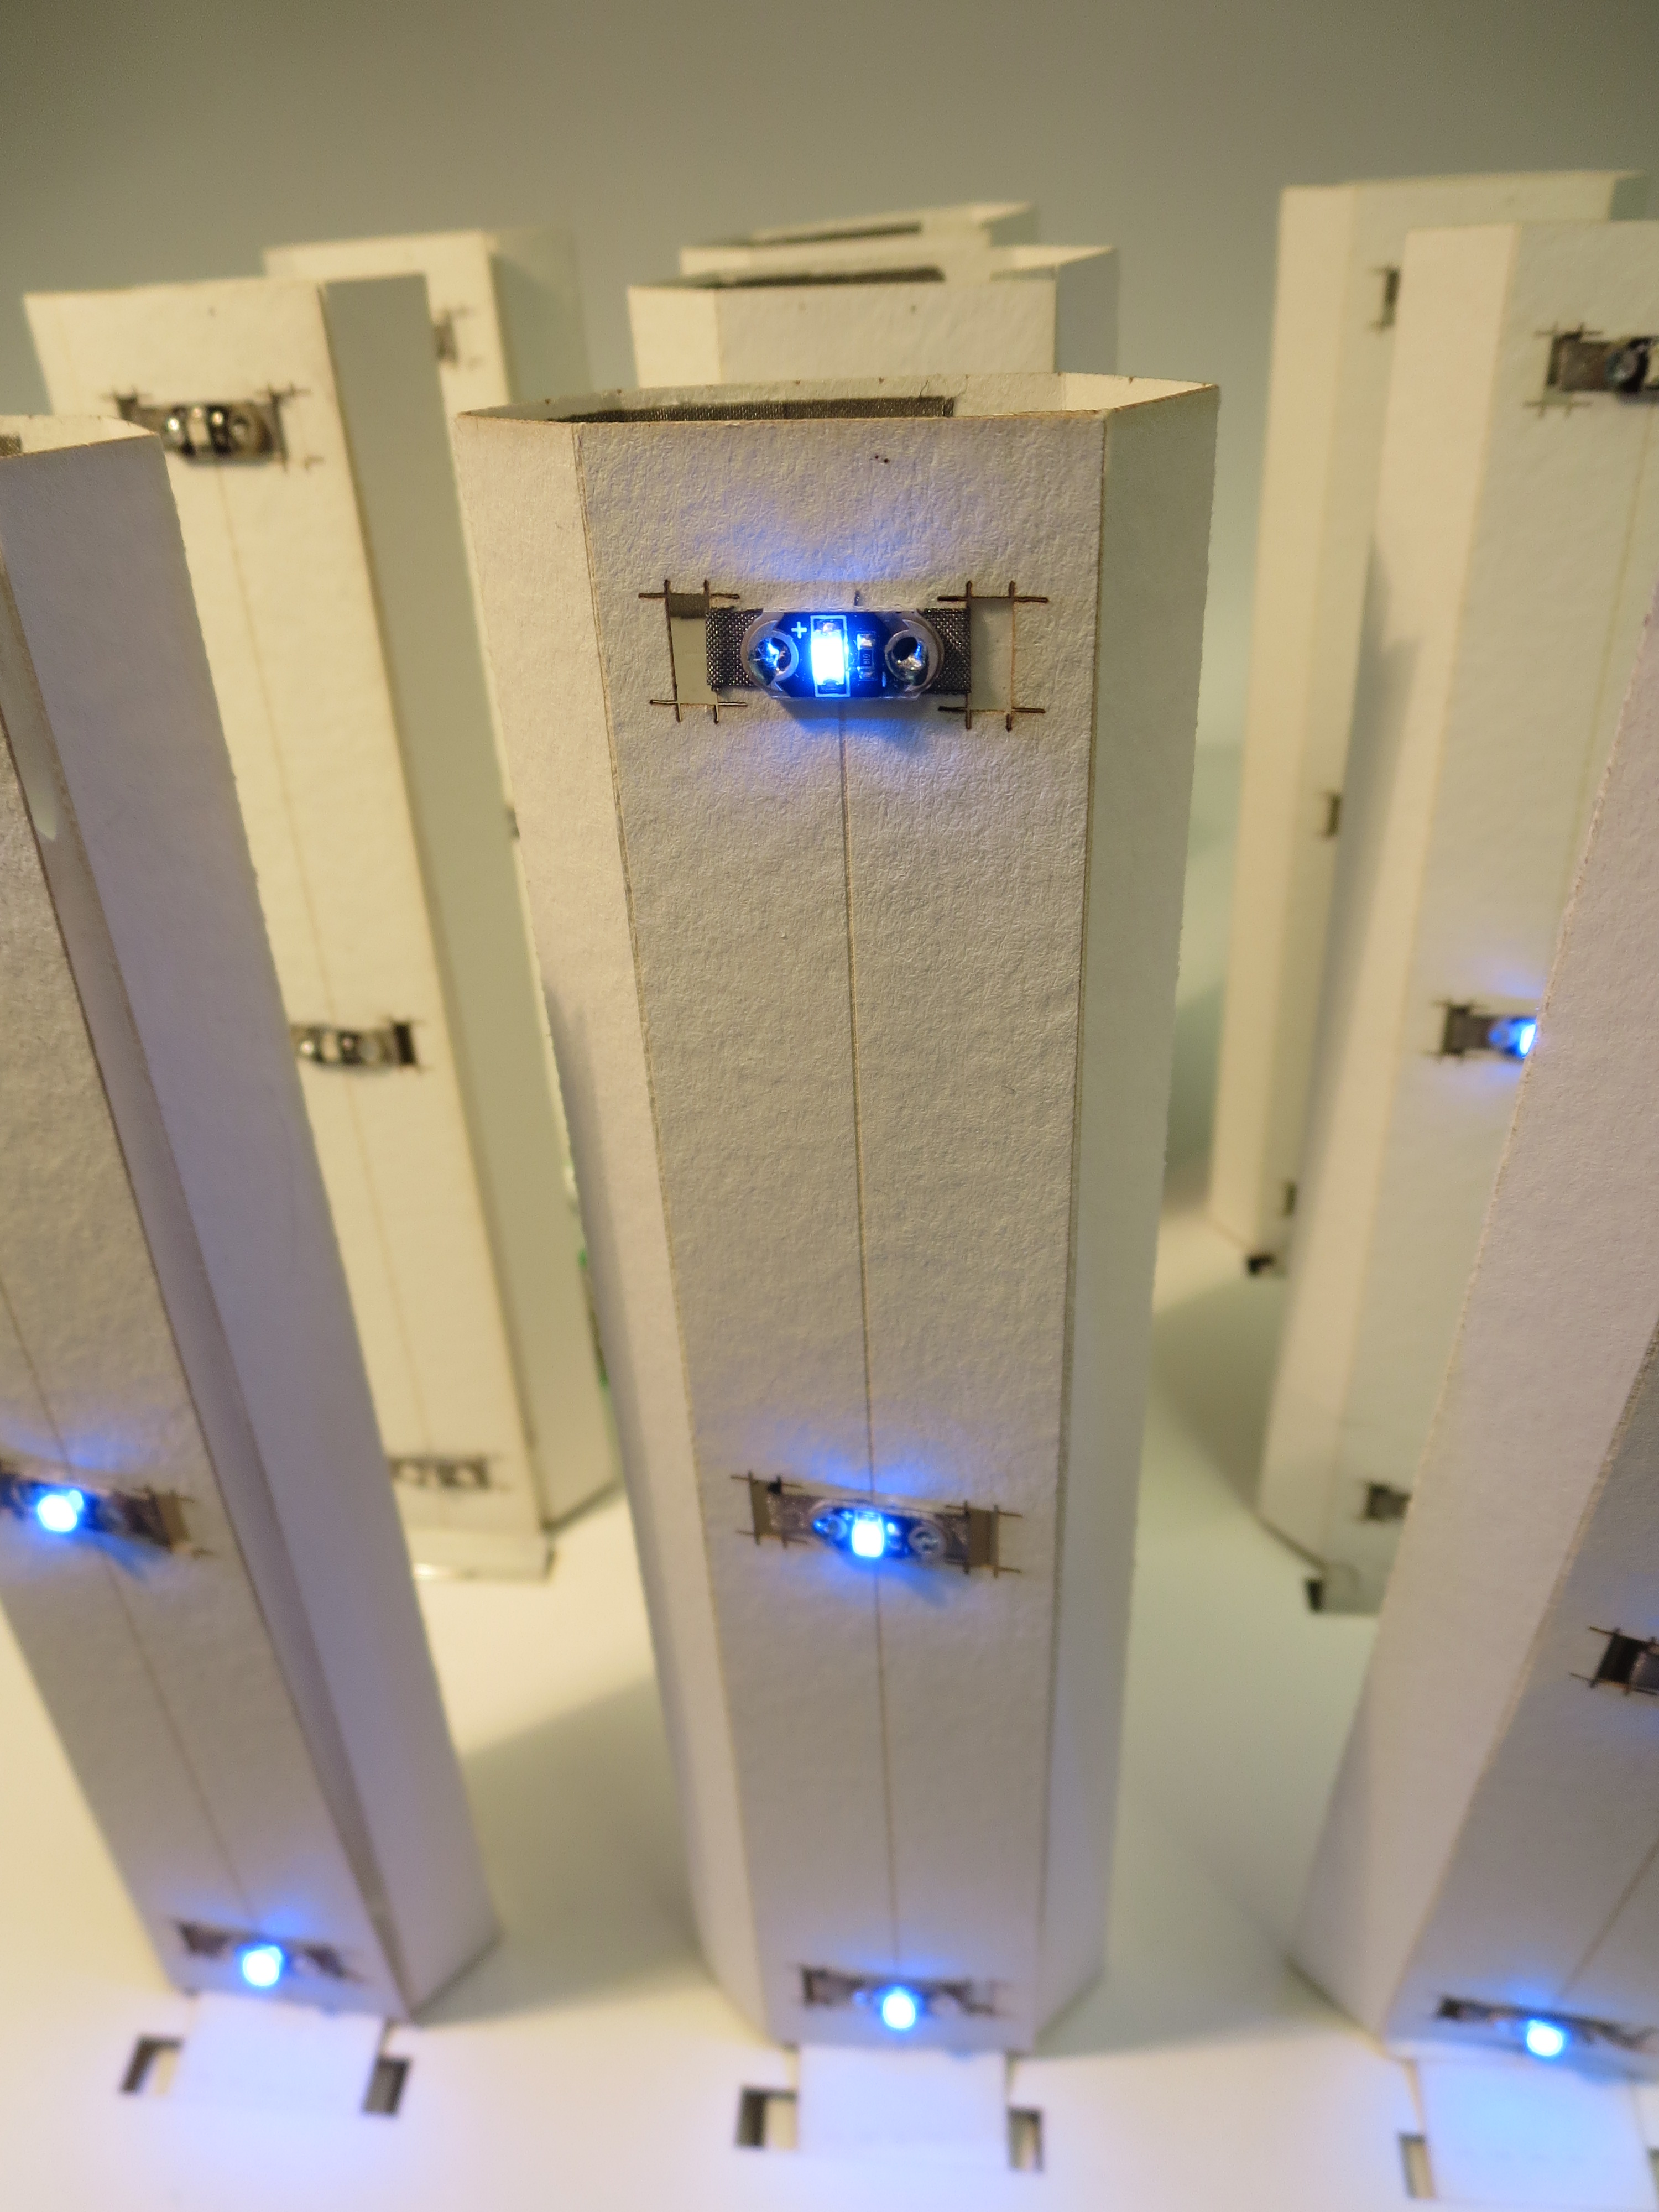
\includegraphics[width=.45\linewidth]{images/pop3}
  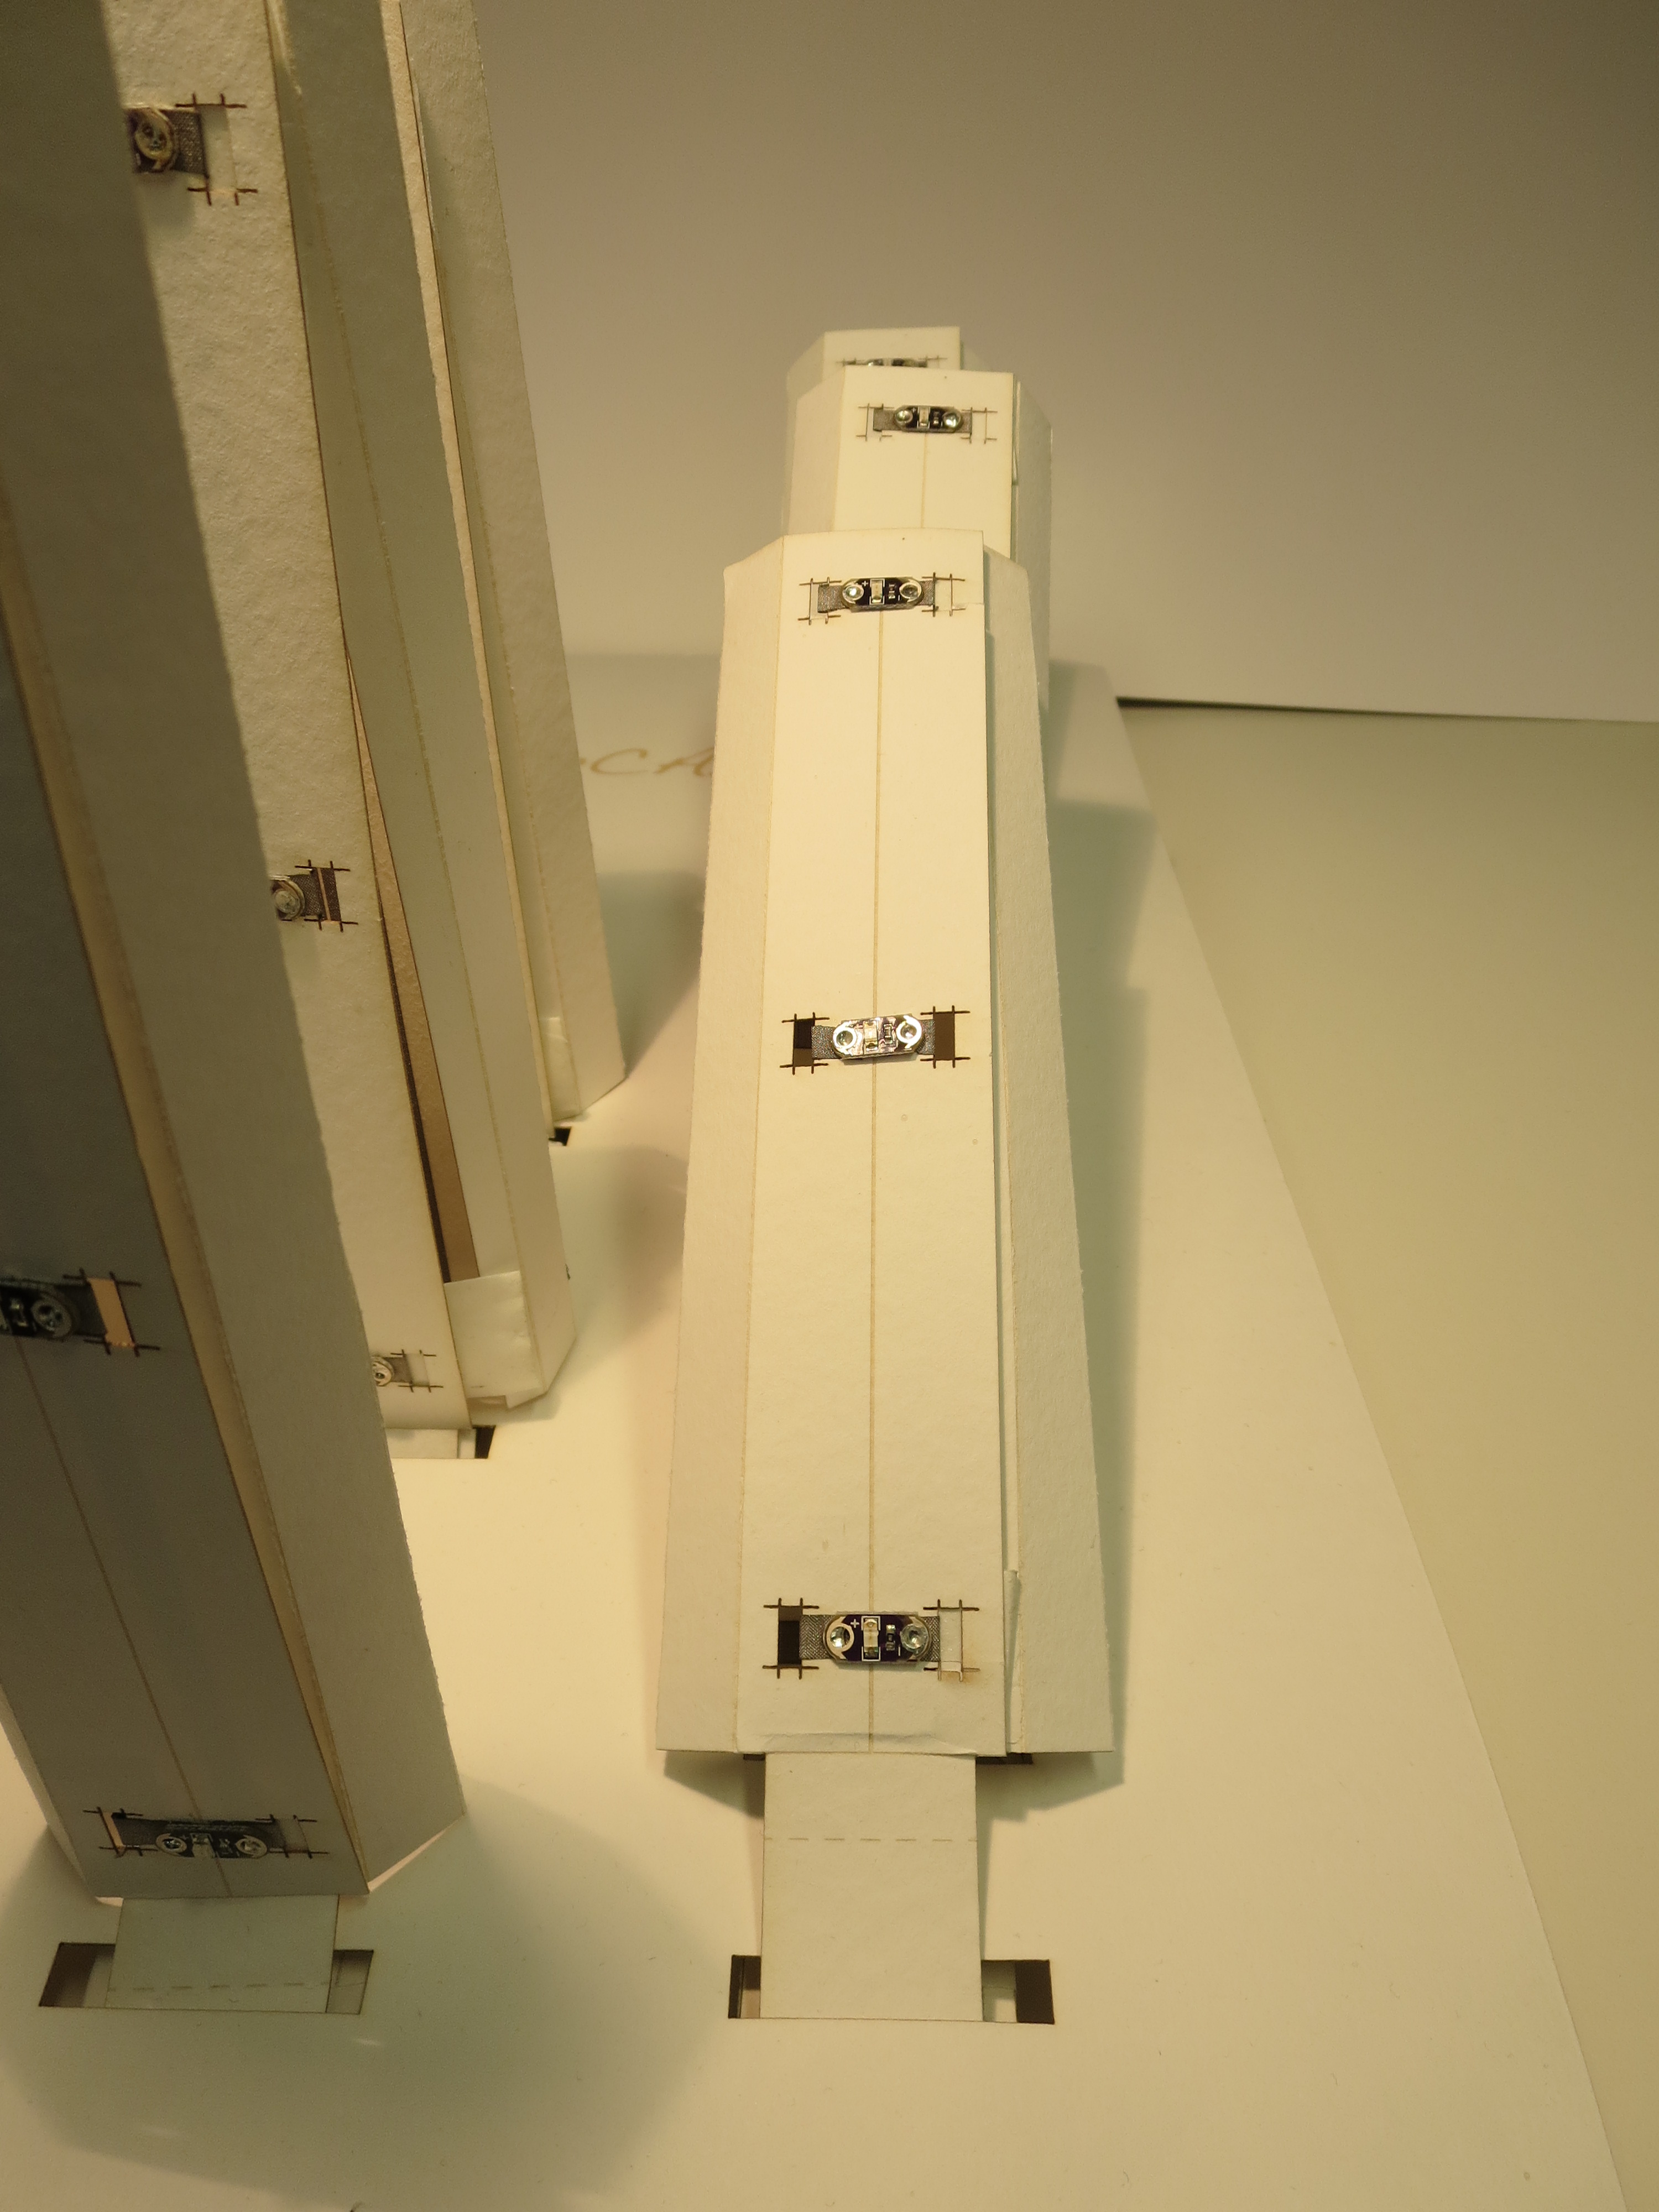
\includegraphics[width=.45\linewidth]{images/popcad_pic2}
  \caption{Two views of PopCADv2 design: with towers raised and LEDs lit
  (left), and with the rightmost column of towers laid flat (right).}
  \label{fig:popcad1}
\end{figure}

\begin{figure}[!ht] 
\begin{center}$
\begin{array}{cc}
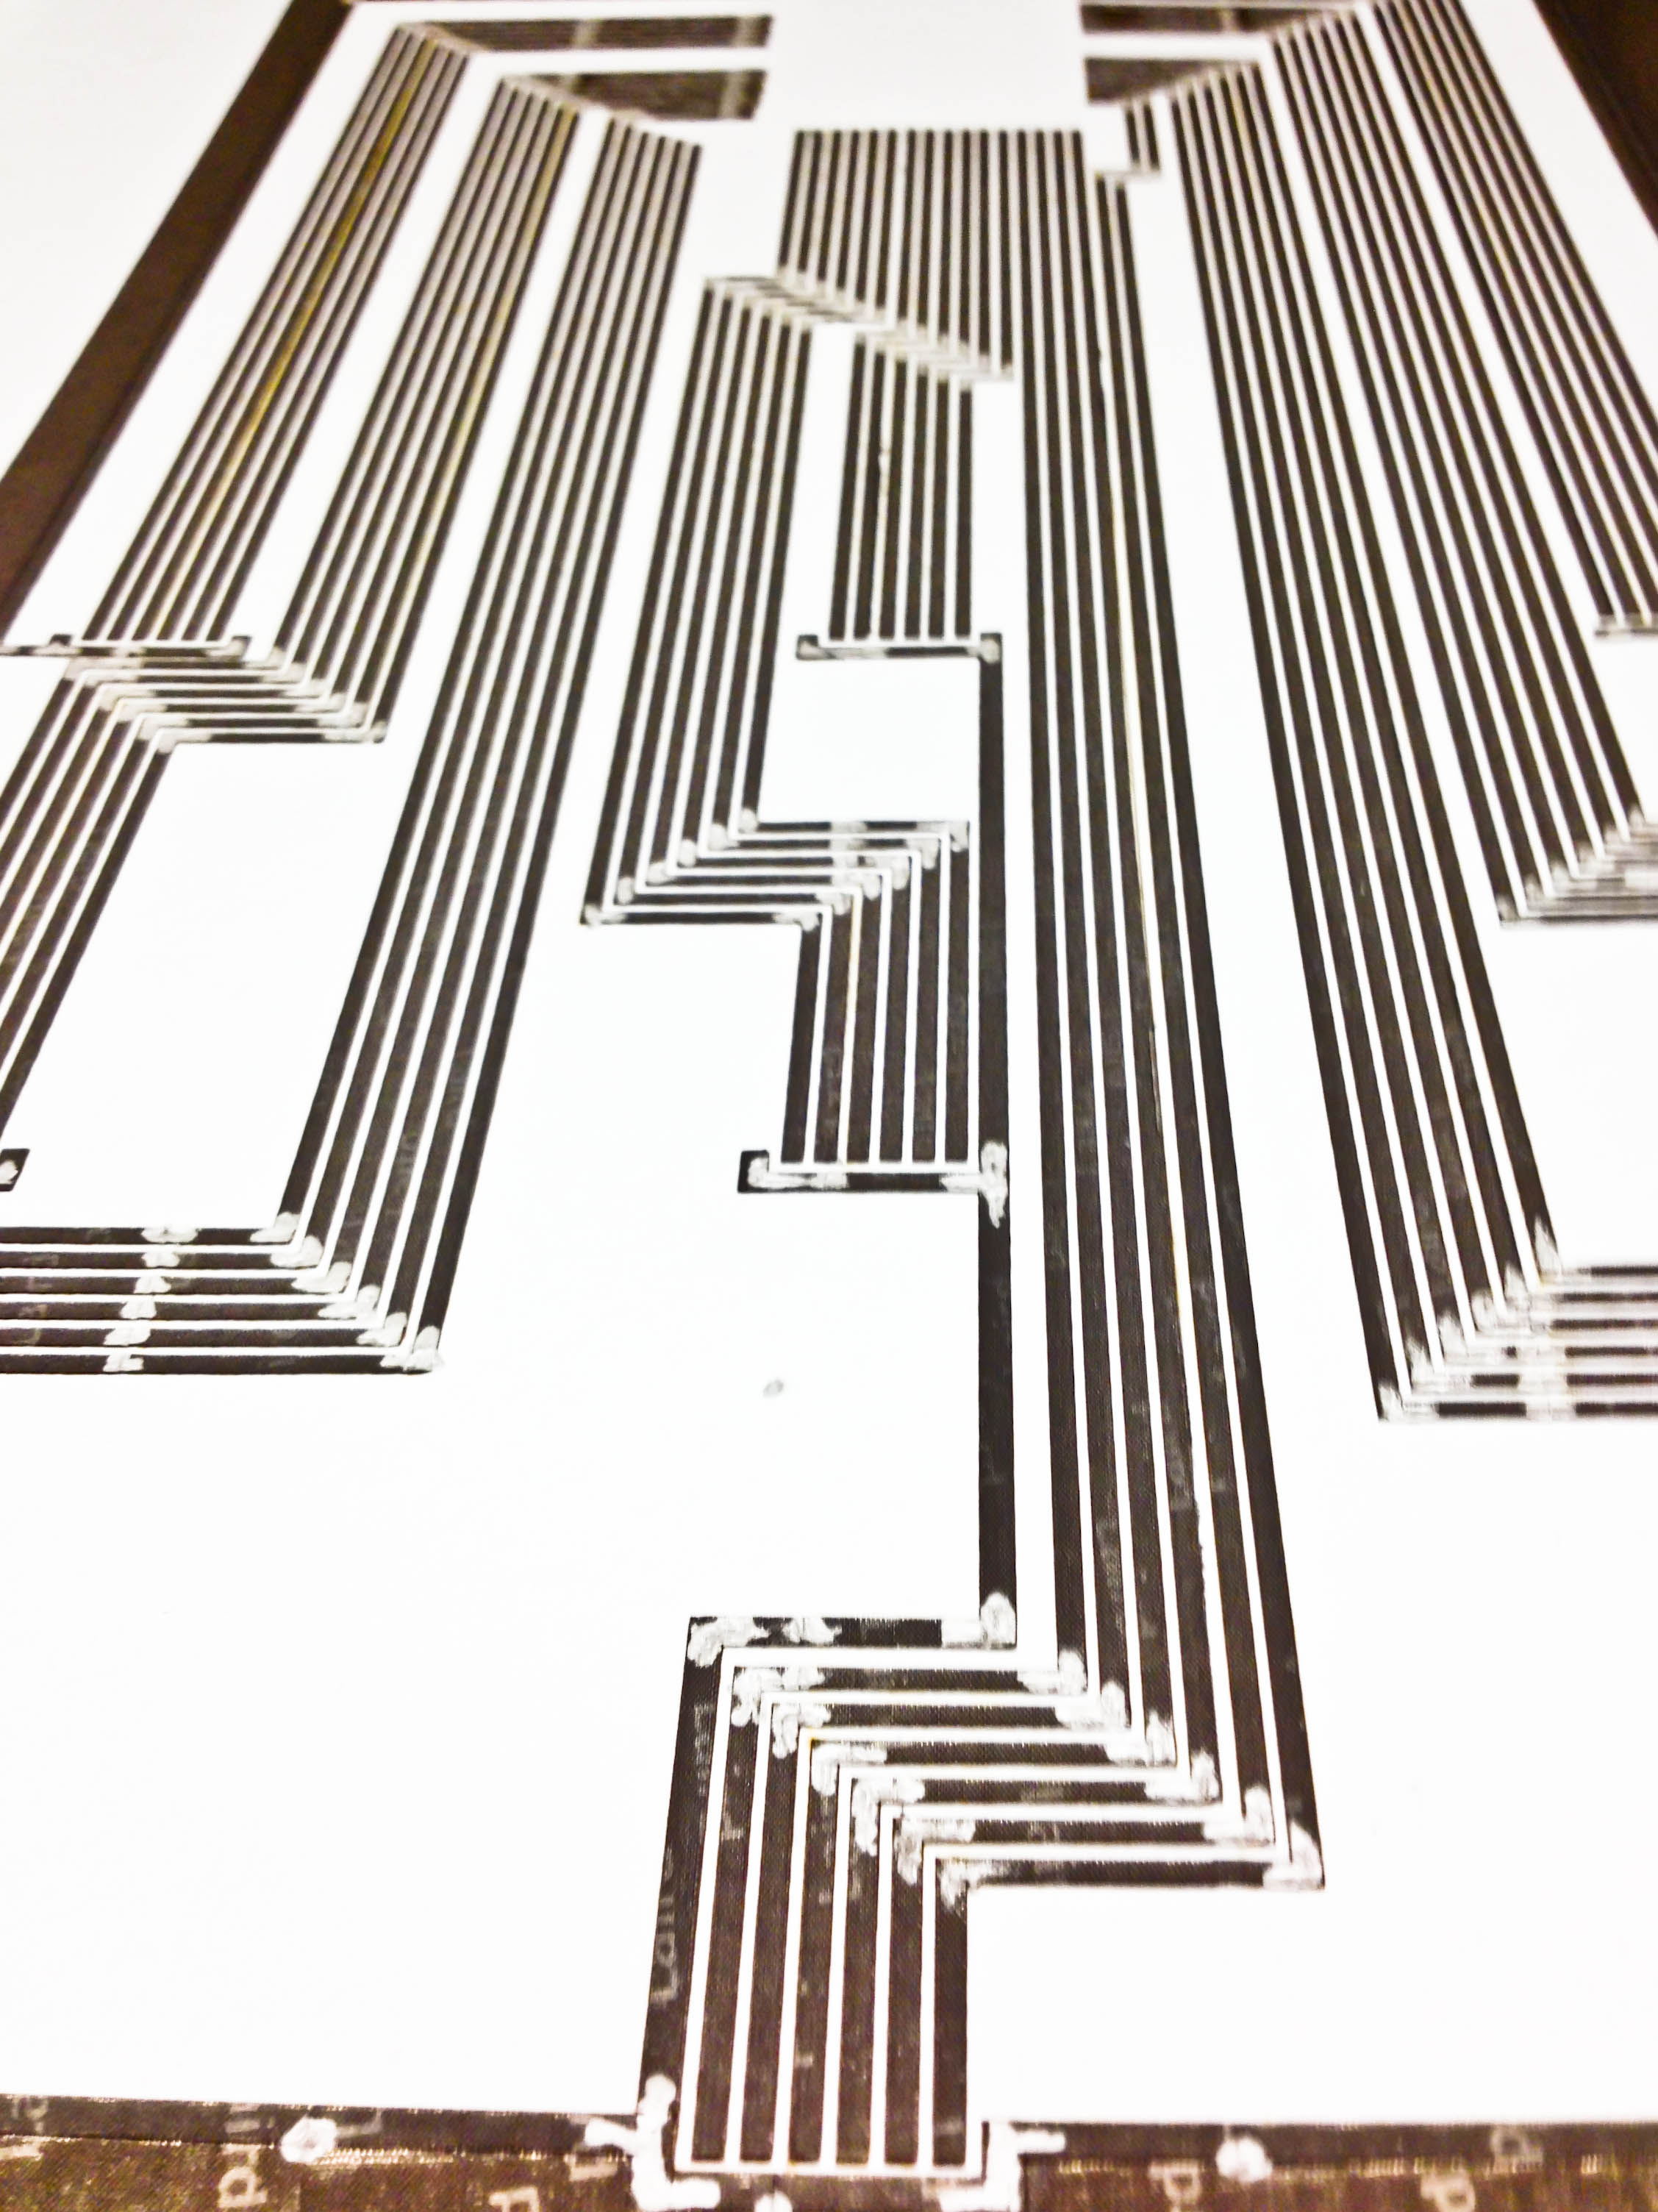
\includegraphics[width=.45\linewidth, height=3.5in]{images/pop_circuit2-2}&
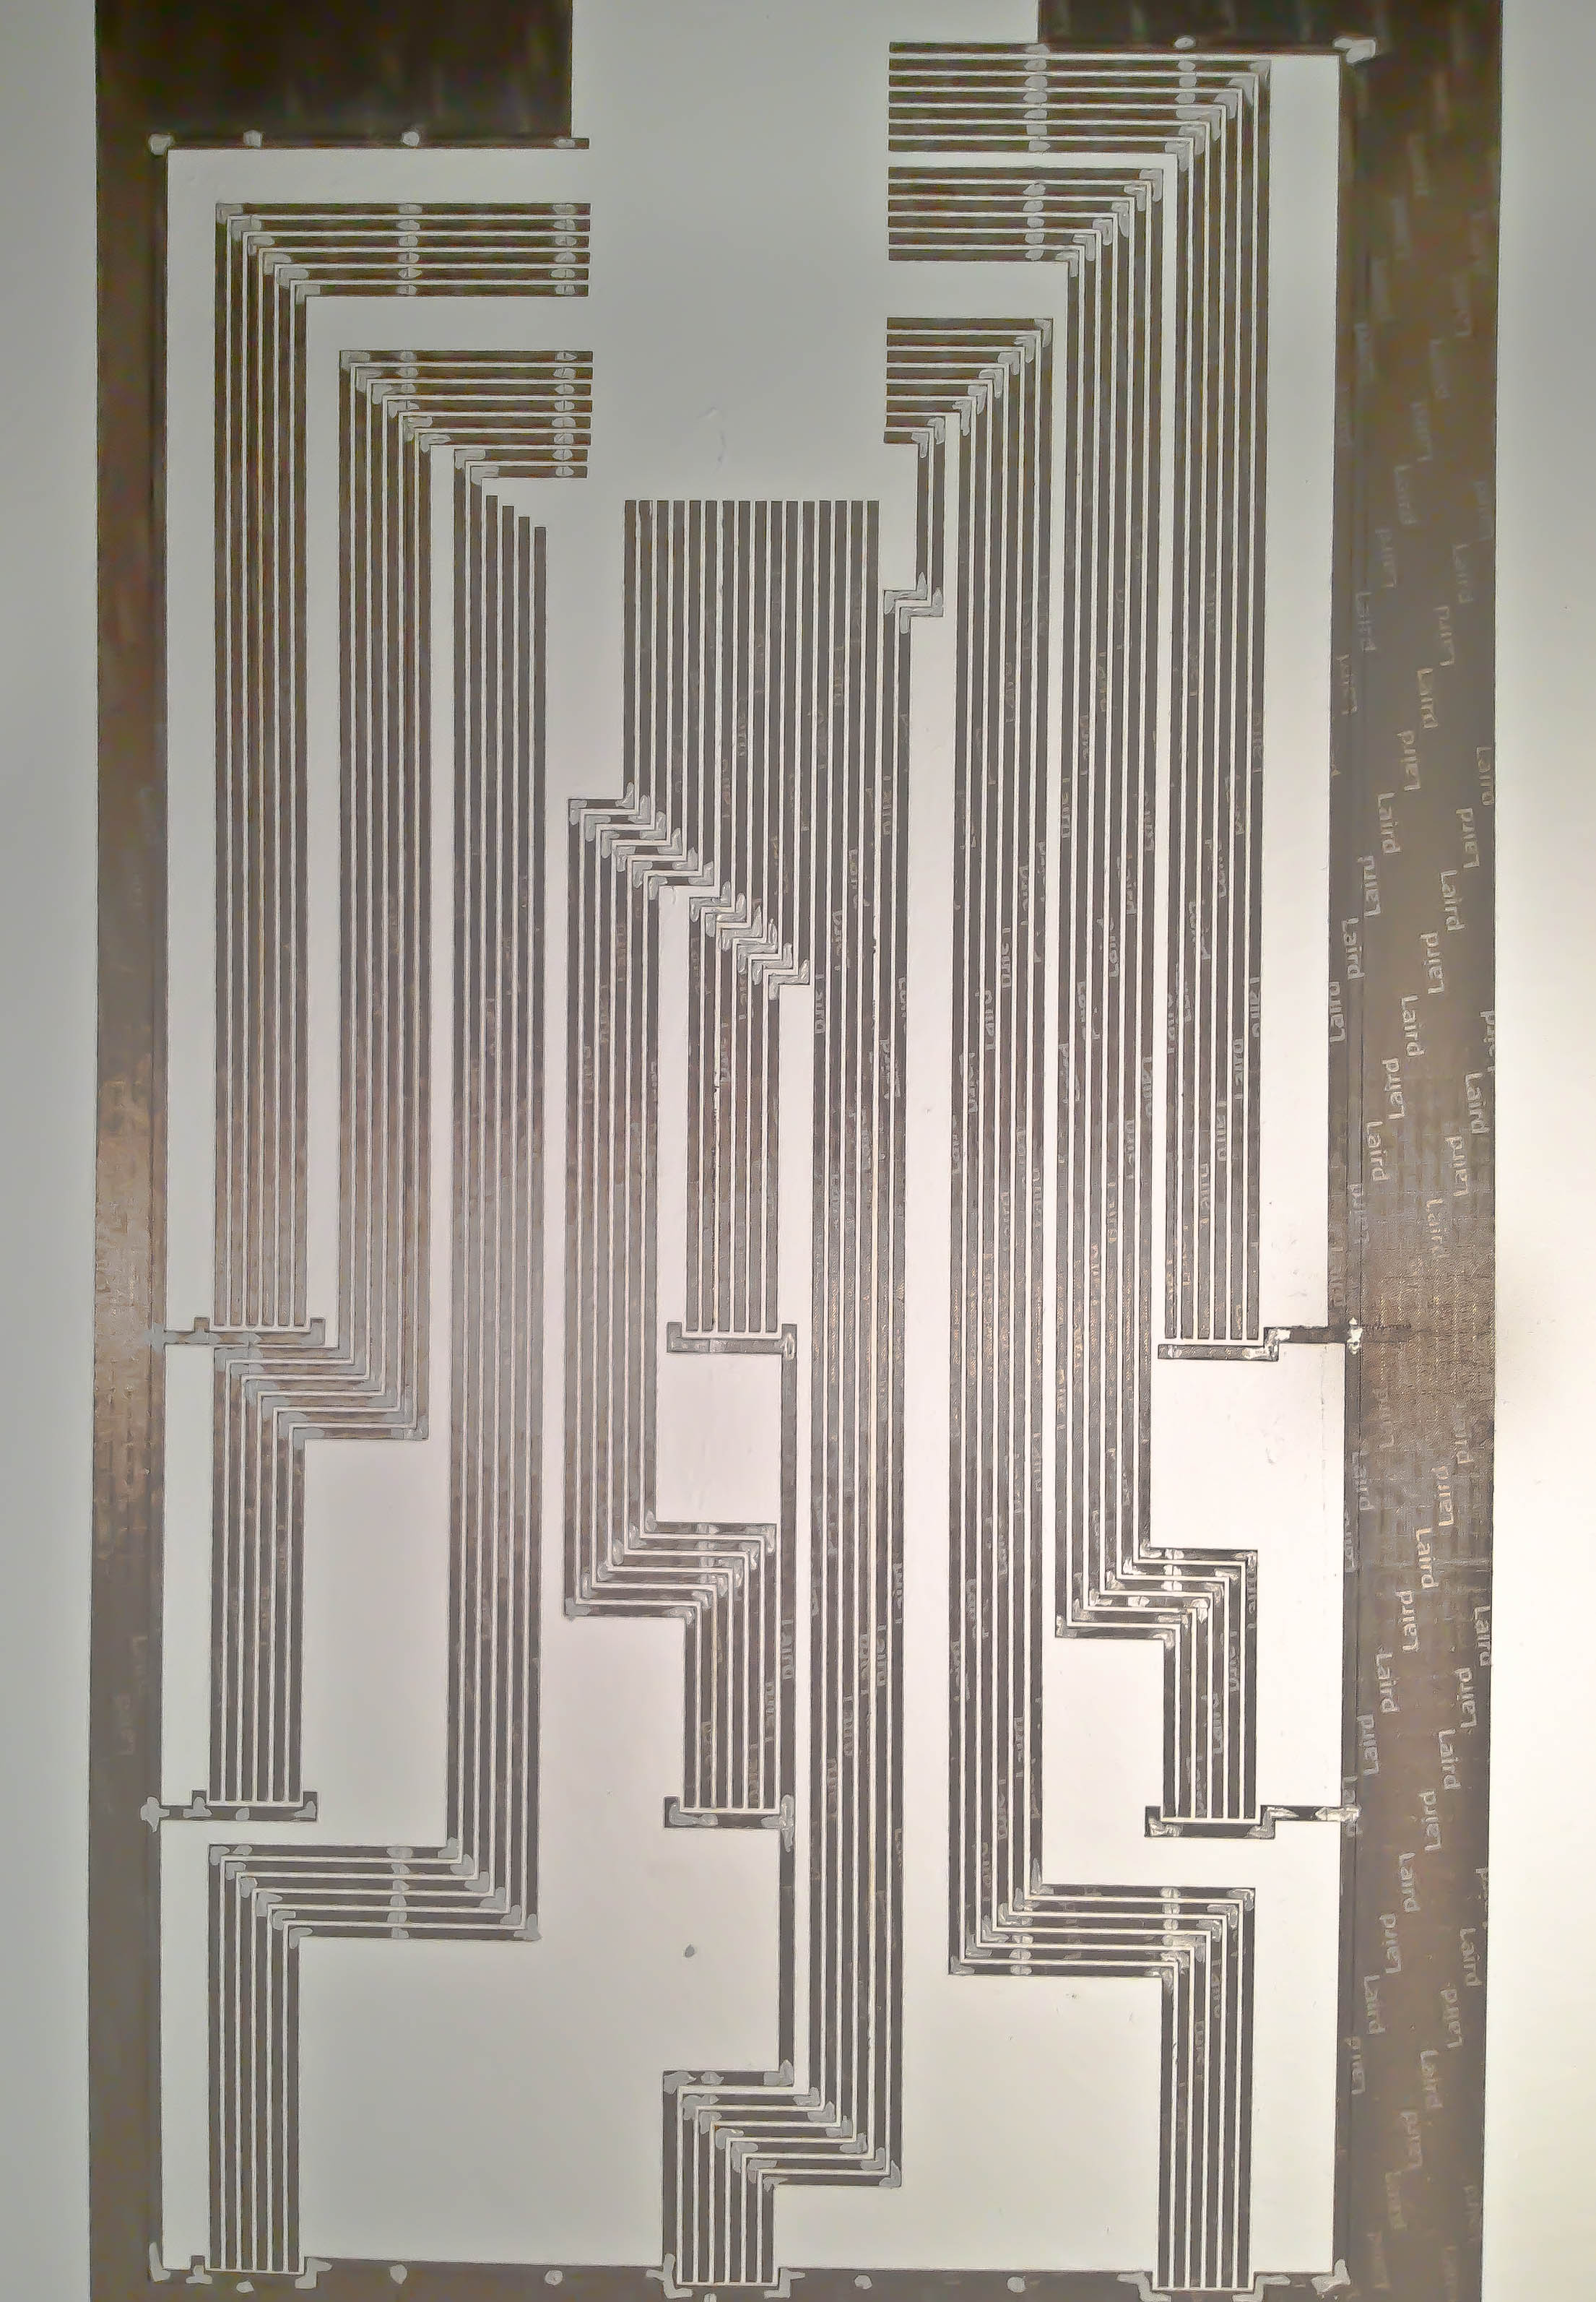
\includegraphics[width=.45\linewidth, height=3.5in]{images/popcad_circuit-3}
\end{array}$
\end{center}
\caption{Two views of the conductive tape circuit connecting the paper towers
to the Arduino Mega microntroller. The circuit was constructed by laser cutting
a design through conductive tape (but not through the paper beneath it) and
removing the excess material.}
\label{fig:popcadCirc}
\end{figure}




\subsection{Discussion}
The software originally written for the UCube and SnapCAD was adapted to work
with the pop-up book, making it capable of similar types of algorithmic modeling
and stereolithography output for 3D printing. As the grid is 3x3x3, it also
makes sense to adapt some of the game-playing aspects of the larger devices
(e.g., it would still be possible to play 3D tic-tac-toe). In addition to adding
this functionality, there are several improvements and finishing touches to be
made on the book itself. Additionally, the current hardware setup for the pop-up
book does not allow for the LED's to be snapped on or off, making certain
multi-player or multi-shape operations impossible. Weather or not this
functionality is crucial to the pop-up book will determine if changes need to be
made.  

Given the different medium of the pop-up book (paper as opposed to circuit
boards), it is worth exploring the possibilities afforded by a cheaper, more
flexible material. For instance, the flexibility of paper might provide the
means for new types of modeling actions. It is plausible to imagine paper tabs
or other mechanisms that perturb the LEDs off the integer lattice, or alter the
overall topology in such a way that new shapes are possible (e.g. by deforming
an equidistant grid into a spherical shape). There may be additional sensors or
hardware that could be embedded into the book to provide new functionality
(rotation, proximity, pressure). Additionally, due the inexpensive and portable
nature of the pop-up book, it is worth exploring the sorts of interactions that
could occur between several pop-up books (e.g., extending the input field to
include two or more grids, networked interactions like cooperative modeling
tasks, or competitive games like 3D-battleship). By using paper as a material to
think with, we may find further possibilities as development continues.

\section{Software}
Put stuff about software development here. Details. Screenshots.

% \subsection{Software}
% 
% The UCube makes use of the Processing\cite{Processing} framework to read in
% the active coordinates from the Arduino microcontroller connected to the
% platform; the software then displays these as larger red points on a grid of
% grey dots. Users can rotate the grid along any axis by clicking and dragging
% with the mouse. In our current early prototype, there are only two buttons on
% the user interface: (i) an �export� button, responsible for taking the current
% set of active points and exporting them into "STL" file format (suitable for 3D
% printers), and (ii) a �mode� button which toggles between showing just the red
% dots as points and filling in an area (defined by a convex hull algorithm) to
% give a sense of shape.
% The software interface is intentionally minimal in order to encourage the user
% to focus on the physical interaction. We felt it was crucial not to fall into
% the trap of making another software tool for experts, so the main purpose of the
% software is to act as an aid�a means to cognitively clarify and confirm the
% user's intentions. Although it is likely that we will extend the software
% somewhat in future iterations, our goal is to support the physical experience of
% specifying a three-dimensional object, and not to add functionality beyond what
% is necessary or helpful to that end.

The UCube Desktop Software The software for the UCube utilizes the Processing
framework to read in the active coordinates from the Arduino microcontroller; it
then displays those coordinates onscreen as larger red points against a grid of
grey dots. This on-screen model can be manipulated in a number of ways. Clicking
and dragging along any axis rotates the model, as does the use of the arrow keys
on the keyboard.  Holding the shift key while performing either action moves the
entire model around the screen (essentially re-centering it). The ``control'' key
plus an up or down arrow key zooms in or out along the z-axis.
In addition to camera movements, there are a limited number of functions
represented by a simple graphical user interface (17 buttons, a slide bar, and
two checkboxes) which aid and expand the modeling capabilities of the UCube:
there are toggles for turning on and off the convex hull of the active points
(either all the points or just the hull of a particular color), viewing the hull
as a wireframe or solid object, and a toggle that shows or hides the background
grid.  In addition, there are several import and export buttons: an export to
STL (stereo lithography) format, the standard format for 3D printer files, as
well as save and load options which allow users to save and re-load their shapes
for use within the UCube system. Figure \ref{fig:software1} shows the UCube
software upon reading in the eight points that were selected in Figure 1: in the
bottom panel, the ``convex hull'' option has been chosen so that a solid cube is
displayed (with the input points visible as the highlighted vertices of the
cube). Now, by exporting this form (as mentioned above) to STL format, and
sending the result to a 3D printer, we can produce a physical model of our
specified shape, as shown in Figure 4.


\begin{figure}[ht] \begin{center}$
\begin{array}{cc}
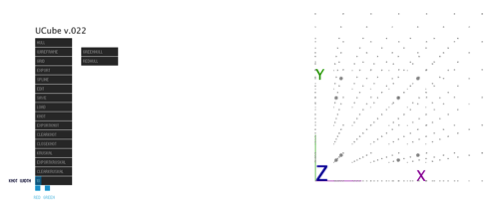
\includegraphics[width=.45\linewidth]{images/software_1} &
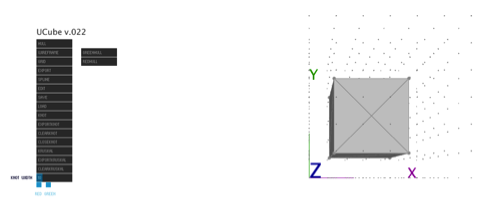
\includegraphics[width=.45\linewidth]{images/software_2}
\end{array}$
\end{center}
\caption{Two screen views (left and right) of the UCube software, illustrating
the way in which the software reads in the points selected in Figure XXXXXX. At
left:
the software is displaying the eight selected spatial points as gray dots. At
right: the software computes the convex hull of the points and produces the
cube designated by the eight selected points in Figure XXXXXX.}
\label{fig:software1}
\end{figure}


Before returning to the software itself, it is worth pointing out that, in
effect, the events depicted in Figures 1, 3, and 4 constitute a typical scenario
for employing the UCube. The user begins by selecting the vertices of a shape
that she wishes to create (Figure 1); checks that shape against its appearance
on the computer screen (Figure 3); and, if satisfied, sends that shape on to be
output by a 3D printing device (Figure 4). There are, of course, limitations to
this scenario - and we will touch upon these in the ensuing discussion.
Nonetheless, it is the overall simplicity of the scenario that originally
inspired the design of the UCube: the user need not construct a shape on a
two-dimensional screen, nor be deeply familiar with the terminology and
operations of modeling software. Instead, the creation of a desired shape takes
place by moving one's hands in space.

To return to the UCube software: while spare in its features, it does allow the
user to perform some operations on the current set of 3D points��operations that
mitigate some of the inherent limitations suggested by the initial scenario just
described. By putting the software in ``edit'' mode, users can click-and-drag
points off the integer lattice, creating shapes that would be impossible with
direct manipulation of the UCube towers. There is also a primitive version of a
``spline'' function, which connects all the active points with a curved spline.
(These are new features, added since the earlier version of the system described
in \cite{Leduc-Mills:2011:UCD:1999030.1999039}.) As a guiding heuristic for our
design, it should be noted that the UCube software is intentionally minimal.
Although there are still some additions to the software that we expect to see
implemented in further iterations (as noted in the final section), our aim is
not to produce another sophisticated software modeling program. Instead, the
software is meant to aid the user in clarifying their physical actions with the
UCube towers and switches.

\subsection{Modeling Modes} 

The previous section described the architecture and implementation of the UCube
2.0. In this section, we outline a variety of 3D design projects that can be
undertaken with the system.






\subsubsection{Convex Hull: Creating Polyhedral Forms} 
The most typical type of 3D modeling done
with the UCube is to create polyhedral forms, such as the cube of Figures 1, 3,
and 4. The basic scenario here is that the user selects a set of locations in
space by placing lights at those locations; much as in Figure 1, the lights can
be interpreted as the outer vertices of a convex shape. The UCube software can
then display and print out the convex hull of the selected

\subsubsection{Points as ``Blocks'': Creating Non-Convex Polyhedral Forms} 
While a ``standard'' UCube project interprets the locations of lights as vertices
of a polyhedron, the device allows for myriad different semantics for spatial
locations. For example, we might wish to interpret the location of a light as
signifying the presence, not of a point, but of a cube in space, centered at the
given location and with an edge-length of one ``hole-interval unit''. By selecting
(say) four successive light locations along the length of one tower, then, one
could specify a rectangular prism (such as the one shown lying horizontally
toward the bottom right of Figure 6). Likewise, by selecting three point
locations in an ``L'' form, one could specify the non-convex polyhedral form seen
at the far left of Figure 6.
The complex form shown toward the back of Figure 6 represents what happens when
we take this idea beyond shapes specified by just a few locations. For those
readers interested in recreational mathematics, seven of the shapes shown in
Figure 6 will be recognizable as the component pieces of the "Soma" puzzle;
these pieces can be arranged together to form a cube. The UCube could be
employed in similar fashion to produce many such dissection-type puzzles.
 
Figure 7. Two ``printed path'' forms created by specifying a temporal sequence of
points with the UCube. The form on the right is a trefoil knot.

\subsubsection{Paths: Creating Linear Forms and Knots} 
In the examples of the previous paragraphs, we have not made use of the fact
that the UCube samples selected points in real time: thus, when a user adds or
subtracts a point in space, that change is registered immediately in the desktop
software. What this means is that the user can exploit not only the overall set
of selected points, but can also make use of the order in which those points are
selected. A sequence of selected points need not represent only vertices of a
solid; it can also represent a path over time in 3D space.
Figure 7 shows a sample project based on this idea. Here, the UCube software has
been employed to read points as successive positions of a path in 3-space. The
resulting paths have been printed out on a 3D printer. In both cases, the path
is closed, finishing at the same location where it started; the path printed out
at right in Figure 7 is in fact a well-known mathematical form, a trefoil knot.
(It may be worth mentioning here that such a knotted form would be rather tricky
to create in standard 3D modeling software, but the form can be created ``by
hand'' with the UCube, selecting light positions in space along the path of the
knot.)

\subsubsection{Point Clouds: Creating Minimal Spanning Trees}
Instead of interpreting points as vertices of a solid (as in the convex hull
examples) or as the successive stations of a temporal path (as in the ``knot''
example above), we could in fact simply treat our set of points as just what
they are�namely, a set of points. Starting with this interpretation, we might
produce a form such as a minimal spanning tree of the set of points (a set of
edges of minimal total length connecting all the points). Figure XXXXX shows an
example of a form created this way: here, the UCube software has computed a
minimal spanning tree from a set of six selected points, and the tree is then
printed out in solid form.

\subsection{Other Software Functionality}
Edit mode, etc.






